\documentclass[13pt,a4paper]{extreport}

% Hướng dẫn dùng XeLaTeX trên Overleaf để hỗ trợ Times New Roman
\usepackage[a4paper,top=2.5cm,bottom=2.5cm,left=3.5cm,right=2cm]{geometry}
\usepackage{fontspec}
\setmainfont{Times New Roman}

\usepackage[unicode]{hyperref}
\usepackage{setspace}
\linespread{1.2}

\usepackage{titlesec}
% Định dạng chương theo chuẩn: CHƯƠNG 1 (giữa, đậm, cỡ 14)
\titleformat{\chapter}[display]
  {\bfseries\centering\fontsize{14pt}{17pt}\selectfont}
  {CHƯƠNG \thechapter}{1ex}{}
\titleformat{\section}{\bfseries\large}{\thesection}{1em}{}
\titleformat{\subsection}{\bfseries\normalsize}{\thesubsection}{1em}{}

% Giảm khoảng trống trước tiêu đề chương để bố cục gọn hơn
\titlespacing*{\chapter}{0pt}{0pt}{18pt}

\usepackage{tocloft}
\renewcommand{\cftchapfont}{\bfseries}
\renewcommand{\cftchappagefont}{\bfseries}
% Đặt cỡ chữ mục lục (các mục, tiểu mục) về \normalsize ~ 13pt
\renewcommand{\cftsecfont}{\normalsize}
\renewcommand{\cftsecpagefont}{\normalsize}
\renewcommand{\cftsubsecfont}{\normalsize}
\renewcommand{\cftsubsecpagefont}{\normalsize}

% Chỉ hiển thị số trang ở giữa chân trang, không có header
\pagestyle{plain}

\setlength{\parindent}{1cm}
\setlength{\parskip}{6pt}

\usepackage{graphicx}
\usepackage{caption}
\usepackage{booktabs}
\usepackage{array}
\usepackage{longtable}
\usepackage{float}

% Đổi nhãn Figure/Table sang Hình/Bảng
\renewcommand{\figurename}{Hình}
\renewcommand{\tablename}{Bảng}

%========================================
% THÔNG TIN ĐỀ TÀI
%========================================
\newcommand{\TenDeTai}{XÂY DỰNG HỆ THỐNG QUẢN LÝ TIỆM CẦM ĐỒ}
\newcommand{\Khoa}{CÔNG NGHỆ THÔNG TIN}
\newcommand{\Truong}{TRƯỜNG ĐẠI HỌC NAM CẦN THƠ}
\newcommand{\SVOne}{Nguyễn Văn Khánh}
\newcommand{\SVTwo}{}
\newcommand{\Lop}{CNTT Kxx}
\newcommand{\GVHD}{ThS.\ ................................}

\begin{document}

%========================================
% BÌA CHÍNH
%========================================
\begin{titlepage}
  \begin{center}
    {\large \Truong}\\[6pt]
    {\large KHOA \Khoa}\\[3cm]

    {\Large\bfseries BÁO CÁO ĐỀ TÀI}\\[1cm]
    {\Large\bfseries \TenDeTai}\\[3cm]

    \begin{tabular}{ll}
      Sinh viên thực hiện: & \SVOne \\
      Lớp:                 & \Lop \\
      GV hướng dẫn:        & \GVHD \\
    \end{tabular}

    \vfill
    {\large Cần Thơ, 2026}
  \end{center}
\end{titlepage}

%========================================
% BÌA PHỤ
%========================================
\begin{titlepage}
  \begin{center}
    {\large \Truong}\\[6pt]
    {\large KHOA \Khoa}\\[3cm]

    {\Large\bfseries BÁO CÁO ĐỀ TÀI}\\[1cm]
    {\Large\bfseries \TenDeTai}\\[3cm]

    \vfill
    {\large Cần Thơ, 2026}
  \end{center}
\end{titlepage}

%========================================
% LỜI CẢM TẠ
%========================================
\pagenumbering{roman}

\chapter*{LỜI CẢM TẠ}
\addcontentsline{toc}{chapter}{LỜI CẢM TẠ}

Trong suốt thời gian học tập tại Trường Đại học Nam Cần Thơ và quá trình thực hiện báo cáo đề tài với nội dung \emph{\TenDeTai}, em đã nhận được rất nhiều sự quan tâm, giúp đỡ từ quý thầy cô, gia đình và bạn bè.

Trước hết, em xin bày tỏ lòng biết ơn sâu sắc đến \GVHD, người đã tận tình hướng dẫn, định hướng và góp ý một cách chi tiết, giúp em định hình được cấu trúc đề tài, tổ chức mã nguồn hợp lý và hoàn thiện nội dung báo cáo.

Em cũng xin chân thành cảm ơn toàn thể quý thầy cô trong khoa \Khoa\ đã tận tâm giảng dạy, truyền đạt cho em kiến thức chuyên môn cũng như những kinh nghiệm thực tiễn quý báu trong suốt thời gian học tập. Đây là nền tảng quan trọng để em có thể vận dụng vào việc xây dựng hệ thống web trong đề tài này.

Bên cạnh đó, em xin gửi lời cảm ơn đến gia đình và bạn bè đã luôn động viên, tạo điều kiện cả về vật chất và tinh thần, là chỗ dựa vững chắc để em yên tâm học tập và nghiên cứu.

Mặc dù em đã cố gắng hoàn thành đề tài một cách tốt nhất, nhưng do hạn chế về thời gian, kinh nghiệm và kiến thức, báo cáo khó tránh khỏi những thiếu sót. Em rất mong nhận được những ý kiến đóng góp của quý thầy cô để có thể hoàn thiện hơn trong tương lai.

\vspace{1cm}
\hfill Cần Thơ, năm 2026

\hfill Sinh viên thực hiện

%========================================
% LỜI CAM ĐOAN
%========================================
\chapter*{LỜI CAM ĐOAN}
\addcontentsline{toc}{chapter}{LỜI CAM ĐOAN}

Em xin cam đoan đề tài \emph{\TenDeTai} là kết quả lao động khoa học của riêng em dưới sự hướng dẫn của \GVHD. Các số liệu, kết quả, hình ảnh, sơ đồ và đoạn mã nguồn trình bày trong báo cáo này là trung thực, được thu thập và xử lý từ quá trình nghiên cứu, phân tích nhu cầu thực tế tại tiệm cầm đồ và cài đặt hệ thống quản lý tiệm cầm đồ dựa trên nền tảng \emph{Flask} và cơ sở dữ liệu \emph{MySQL}. Những tài liệu tham khảo, nội dung trích dẫn từ các nguồn khác đều được trích dẫn rõ ràng trong phần Tài liệu tham khảo.

Sinh viên hoàn toàn chịu trách nhiệm trước nhà trường về lời cam đoan này.

\vspace{1cm}
\hfill Cần Thơ, năm 2026

\hfill Sinh viên thực hiện

%========================================
% NHẬN XÉT CƠ QUAN THỰC TẬP
%========================================
\chapter*{NHẬN XÉT CỦA CƠ QUAN THỰC TẬP}
\addcontentsline{toc}{chapter}{NHẬN XÉT CỦA CƠ QUAN THỰC TẬP}

% (Để trống để in và xin nhận xét)

%========================================
% MỤC LỤC, DANH MỤC
%========================================
\tableofcontents
\addcontentsline{toc}{chapter}{MỤC LỤC}
\clearpage

\listoftables
\addcontentsline{toc}{chapter}{DANH MỤC BẢNG}
\clearpage

\listoffigures
\addcontentsline{toc}{chapter}{DANH MỤC HÌNH}
\clearpage

\chapter*{DANH MỤC TỪ VIẾT TẮT}
\addcontentsline{toc}{chapter}{DANH MỤC TỪ VIẾT TẮT}

\begin{longtable}{p{3cm}p{10cm}}
  DFD   & Data Flow Diagram (Sơ đồ luồng dữ liệu)\\
  ERD   & Entity Relationship Diagram (Sơ đồ thực thể -- liên kết)\\
  ORM   & Object--Relational Mapping (Kỹ thuật ánh xạ đối tượng--quan hệ)\\
  REST  & Representational State Transfer (Phong cách kiến trúc dịch vụ web)\\
  CRUD  & Create, Read, Update, Delete (Các thao tác dữ liệu cơ bản)\\
\end{longtable}

%========================================
% NỘI DUNG CHÍNH
%========================================
\clearpage
\pagenumbering{arabic}

%---------------------------------------
\chapter{GIỚI THIỆU}
%---------------------------------------

\section{Lý do chọn đề tài}

Trong thực tế hoạt động kinh doanh tại các tiệm cầm đồ, việc quản lý thông tin khách hàng, tài sản cầm cố, số tiền gốc và tiền lãi theo từng kỳ luôn là vấn đề phức tạp và tiềm ẩn nhiều rủi ro. Nhiều cơ sở vẫn lựa chọn hình thức ghi chép thủ công bằng sổ tay hoặc sử dụng các file bảng tính rời rạc. Cách làm này có thể tạm chấp nhận ở giai đoạn đầu khi số lượng khách và số lượng phiếu cầm còn ít, nhưng khi quy mô giao dịch tăng lên thì những hạn chế dần bộc lộ rõ rệt: số liệu dễ sai lệch, khó truy vết lịch sử, khó tổng hợp báo cáo, đồng thời việc phát hiện các phiếu đến hạn hoặc quá hạn chủ yếu dựa vào kinh nghiệm và trí nhớ của nhân viên.

Thực tế cho thấy, chỉ cần một sai sót nhỏ trong khâu ghi chép cũng có thể dẫn đến tranh chấp giữa tiệm và khách hàng về số tiền đã vay, số kỳ lãi đã đóng hoặc thời điểm đến hạn chuộc. Trong bối cảnh cạnh tranh ngày càng tăng, khách hàng có xu hướng so sánh mức độ chuyên nghiệp giữa các tiệm cầm đồ; nếu quy trình xử lý nghiệp vụ thiếu minh bạch, chủ tiệm rất dễ mất uy tín, thậm chí có nguy cơ đối mặt với rủi ro pháp lý khi không chứng minh được tính chính xác của thông tin giao dịch. Ngoài ra, việc tổng hợp số liệu cuối ngày, cuối tháng để đánh giá tình hình kinh doanh cũng tốn nhiều thời gian và phụ thuộc nhiều vào kinh nghiệm cá nhân của người làm sổ sách.

Bên cạnh áp lực về hiệu quả kinh doanh, hoạt động cầm đồ còn chịu sự điều chỉnh chặt chẽ của pháp luật. Mỗi phiếu cầm phải có đầy đủ thông tin về khách hàng, giấy tờ tùy thân, tài sản cầm cố, số tiền, lãi suất, thời hạn, lịch sử thu lãi và thời điểm tất toán. Khi quản lý bằng sổ sách, việc tìm kiếm một phiếu bất kỳ theo mã phiếu, theo khách hàng hoặc theo khoảng thời gian thường mất rất nhiều thời gian, dễ xảy ra nhầm lẫn hoặc bỏ sót. Điều này không chỉ ảnh hưởng đến uy tín của tiệm trong mắt khách hàng mà còn gây khó khăn khi cơ quan chức năng cần kiểm tra, đối chiếu hồ sơ giao dịch trong một giai đoạn nhất định.

Trong bối cảnh đó, việc xây dựng một hệ thống phần mềm quản lý tiệm cầm đồ chuyên biệt, được thiết kế xoay quanh các nghiệp vụ thực tế như lập phiếu cầm, thu lãi định kỳ, gia hạn, tất toán, báo cáo doanh thu và quản lý nhân viên là hết sức cần thiết. Hệ thống không chỉ giúp chuẩn hóa quy trình xử lý nghiệp vụ, giảm phụ thuộc vào trí nhớ cá nhân mà còn góp phần nâng cao tính minh bạch của hoạt động kinh doanh, bảo vệ quyền lợi hợp pháp của cả tiệm và khách hàng. Hơn nữa, khi nhu cầu mở rộng quy mô hoặc thành lập thêm chi nhánh xuất hiện, một nền tảng phần mềm tương đối hoàn chỉnh sẽ là điều kiện tiên quyết để đảm bảo khả năng quản lý tập trung và đồng bộ dữ liệu.

Xuất phát từ những lý do trên, nhóm quyết định chọn đề tài \emph{\TenDeTai} với mong muốn xây dựng một hệ thống web gọn nhẹ, phù hợp với một tiệm cầm đồ cỡ vừa, đồng thời có khả năng mở rộng trong tương lai. Thông qua đề tài, nhóm không chỉ mong muốn vận dụng kiến thức đã học về lập trình web, cơ sở dữ liệu và phân tích thiết kế hệ thống vào một bài toán thực tế, mà còn kỳ vọng đề xuất được một mô hình giải pháp có thể áp dụng cho nhiều tiệm cầm đồ nhỏ lẻ khác trên địa bàn, góp phần hỗ trợ số hóa hoạt động quản lý ở lĩnh vực vốn còn ít được tự động hóa này.

\section{Mục tiêu đề tài}

\subsection{Mục tiêu tổng quát}

Mục tiêu tổng quát của đề tài là xây dựng một hệ thống web giúp tin học hóa toàn bộ hoạt động quản lý của một tiệm cầm đồ, từ khâu tiếp nhận khách hàng, lập phiếu cầm, thu lãi, gia hạn, tất toán cho đến báo cáo doanh thu và quản lý nhân viên. Hệ thống được thiết kế theo kiến trúc client--server, trong đó lớp giao diện người dùng được xây dựng bằng \emph{Flask} kết hợp \emph{HTML/CSS} và \emph{TailwindCSS}, còn dữ liệu được lưu trữ tập trung trên \emph{MySQL} và được truy xuất thông qua ORM \emph{SQLAlchemy}. Thông qua hệ thống, chủ tiệm và nhân viên có thể theo dõi tình trạng các phiếu cầm theo thời gian thực, hạn chế tối đa sai sót do ghi chép thủ công và nâng cao tính chuyên nghiệp trong giao dịch với khách hàng.

\subsection{Mục tiêu cụ thể}

Về mặt cụ thể, đề tài hướng tới các mục tiêu sau. Thứ nhất, thiết kế được mô hình dữ liệu phản ánh đầy đủ các thực thể và mối quan hệ quan trọng trong hoạt động của tiệm cầm đồ, bao gồm khách hàng, tài sản cầm cố, phiếu cầm, các lần thu lãi, các lần gia hạn, lần tất toán và nhân viên thực hiện. Mô hình dữ liệu phải bảo đảm tính nhất quán và dễ mở rộng khi bổ sung thêm nghiệp vụ trong tương lai.

Thứ hai, hiện thực một ứng dụng web với các chức năng chính: quản lý thông tin khách hàng (kèm giấy tờ tùy thân), quản lý tài sản cầm cố, lập phiếu cầm, tính lãi đến một thời điểm bất kỳ, ghi nhận các lần thu lãi, gia hạn phiếu, tất toán phiếu, in phiếu cầm và phiếu chuộc. Đề tài cũng tích hợp cơ chế thanh toán qua mã \emph{QR} ngân hàng để hỗ trợ khách hàng chuyển khoản, với nội dung và số tiền được sinh tự động theo từng phiếu.

Thứ ba, xây dựng cơ chế phân quyền giữa hai nhóm người dùng chính là quản trị viên và nhân viên giao dịch. Nhân viên chỉ được thao tác trong phạm vi nghiệp vụ được giao, trong khi quản trị viên có thêm quyền quản lý nhân viên, khóa/mở tài khoản, đặt lại mật khẩu, cấu hình một số tham số hệ thống và xem báo cáo tổng hợp doanh thu gốc, doanh thu lãi theo thời gian.

Thứ tư, cung cấp các báo cáo trực quan về doanh thu gốc, doanh thu lãi, số lượng phiếu đang cầm, số phiếu quá hạn và danh sách phiếu đến hạn trong ngày. Báo cáo được thể hiện dưới dạng bảng và biểu đồ bằng \emph{Chart.js}, giúp chủ tiệm có cái nhìn tổng quan về hoạt động kinh doanh để đưa ra các quyết định điều chỉnh lãi suất, thời hạn cầm hoặc chính sách chăm sóc khách hàng.

\section{Phạm vi và phương pháp nghiên cứu}

Đề tài tập trung vào việc xây dựng hệ thống quản lý cho một tiệm cầm đồ đơn lẻ, chưa xét đến bài toán liên thông nhiều chi nhánh hoặc tích hợp với các hệ thống bên ngoài như phần mềm kế toán, hệ thống CRM tổng thể hay cổng thanh toán ngân hàng. Việc giới hạn phạm vi như vậy giúp nhóm có thể tập trung đi sâu vào các nghiệp vụ trọng tâm của một tiệm cầm đồ điển hình, tránh dàn trải nguồn lực vào những vấn đề quá rộng so với khuôn khổ báo cáo đề tài. Các nghiệp vụ được xem xét bao gồm: quản lý khách hàng, quản lý tài sản cầm cố, lập phiếu cầm, thu lãi theo kỳ, gia hạn phiếu, tất toán phiếu, khóa/mở tài khoản nhân viên và báo cáo doanh thu; các nghiệp vụ khác như xử lý tài sản thanh lý, tích hợp dịch vụ bên ngoài được xem là hướng phát triển trong tương lai.

Về mặt kỹ thuật, hệ thống sử dụng ngôn ngữ \emph{Python} và thư viện \emph{Flask} để xây dựng lớp web, kết hợp với \emph{Jinja2} cho phần template giao diện. Cơ sở dữ liệu được triển khai trên \emph{MySQL} với ORM \emph{SQLAlchemy}. Phần giao diện sử dụng \emph{TailwindCSS} giúp việc xây dựng các thành phần UI trở nên nhanh chóng nhưng vẫn bảo đảm tính nhất quán và hiện đại. Ngoài ra, nhóm còn sử dụng \emph{Selenium} để tự động hóa một số kịch bản kiểm thử giao diện và chụp hình minh họa hệ thống phục vụ cho báo cáo. Toàn bộ mã nguồn được tổ chức trong một project Flask duy nhất, thuận tiện cho việc triển khai trên máy chủ hoặc máy trạm dùng chung trong môi trường phòng máy.

Phương pháp nghiên cứu được lựa chọn theo hướng kết hợp giữa nghiên cứu tài liệu, khảo sát thực tế và thực nghiệm kỹ thuật. Trước hết, nhóm tiến hành tìm hiểu các quy định pháp luật liên quan đến hoạt động cầm cố tài sản, các tài liệu mô tả nghiệp vụ cầm đồ và tham khảo quy trình làm việc tại một tiệm cầm đồ cụ thể. Trên cơ sở đó, nhóm tổ chức các buổi trao đổi ngắn với chủ tiệm và nhân viên giao dịch để làm rõ thêm các bước nghiệp vụ, các tình huống phát sinh trong thực tế mà tài liệu lý thuyết chưa phản ánh đầy đủ.

Tiếp theo, nhóm sử dụng các kỹ thuật phân tích và mô hình hóa hệ thống quen thuộc trong lĩnh vực công nghệ thông tin. Yêu cầu chức năng và phi chức năng được tổng hợp và trình bày lại dưới dạng Use Case, từ đó xây dựng các sơ đồ Use Case, sơ đồ luồng dữ liệu (DFD), sơ đồ thực thể--liên kết (ERD) và sơ đồ lớp. Những mô hình này không chỉ hỗ trợ việc hình dung cấu trúc và luồng xử lý của hệ thống mà còn đóng vai trò như tài liệu trao đổi với người dùng và giảng viên hướng dẫn trong quá trình rà soát yêu cầu.

Cuối cùng, hệ thống được cài đặt thử nghiệm dựa trên các mô hình đã xây dựng. Nhóm triển khai hệ thống trên môi trường phát triển, sử dụng dữ liệu giả lập gần với thực tế, xây dựng các kịch bản kiểm thử phản ánh các tình huống nghiệp vụ điển hình như lập phiếu cầm, thu lãi nhiều kỳ, gia hạn và tất toán phiếu, xử lý trường hợp phiếu quá hạn. Kết quả kiểm thử được đối chiếu với yêu cầu ban đầu để đánh giá mức độ đáp ứng của hệ thống, đồng thời ghi nhận những hạn chế và đề xuất hướng phát triển trong tương lai.

\section{Cấu trúc báo cáo đề tài}

Báo cáo đề tài được bố cục thành bảy chương liên kết chặt chẽ với nhau. Chương~1 trình bày lý do chọn đề tài, mục tiêu, phạm vi và phương pháp nghiên cứu, đồng thời phác họa bối cảnh hoạt động của tiệm cầm đồ trong thực tế. Chương~2 trình bày cơ sở lý thuyết và các công nghệ được sử dụng trong đề tài như Python, Flask, SQLAlchemy, MySQL và TailwindCSS. Chương~3 tập trung vào phân tích và thiết kế hệ thống, mô tả các yêu cầu chức năng, phi chức năng, xây dựng sơ đồ Use Case, sơ đồ luồng dữ liệu, sơ đồ thực thể--liên kết và sơ đồ lớp cho hệ thống quản lý tiệm cầm đồ. Chương~4 trình bày kiến trúc tổng thể của hệ thống, cách tổ chức mã nguồn Flask, chi tiết các module chính và cách xử lý những nghiệp vụ cốt lõi như lập phiếu cầm, thu lãi, gia hạn, tất toán cũng như xử lý trạng thái phiếu. Chương~5 minh họa giao diện người dùng và luồng thao tác của nhân viên, sử dụng các hình chụp màn hình được tự động hóa bằng Selenium để minh họa cho từng chức năng chính trên hệ thống. Chương~6 đánh giá hệ thống dựa trên các kịch bản kiểm thử thực nghiệm, phân tích ưu điểm và hạn chế. Cuối cùng, Chương~7 đưa ra kết luận, nêu các hạn chế còn tồn tại và đề xuất một số hướng phát triển hệ thống trong tương lai như hỗ trợ đa chi nhánh, tích hợp thanh toán trực tuyến và xây dựng ứng dụng di động dành cho chủ tiệm.

%---------------------------------------
\chapter{CƠ SỞ LÝ THUYẾT VÀ CÔNG NGHỆ}
%---------------------------------------

\section{Kiến trúc client--server và ứng dụng web}

Hệ thống quản lý tiệm cầm đồ trong đề tài được xây dựng theo mô hình client--server cổ điển, trong đó trình duyệt web đóng vai trò client, gửi các yêu cầu HTTP tới máy chủ ứng dụng Flask. Máy chủ chịu trách nhiệm xử lý nghiệp vụ, truy xuất cơ sở dữ liệu MySQL và trả về trang HTML đã được render sẵn cho client. Cách tiếp cận này tận dụng những ưu điểm quen thuộc của ứng dụng web: người dùng chỉ cần một trình duyệt hiện đại để truy cập, không phải cài đặt thêm phần mềm trên máy trạm; việc nâng cấp hệ thống được thực hiện tập trung trên máy chủ, giảm chi phí bảo trì và triển khai.

Về mặt kỹ thuật, các request từ trình duyệt được gửi theo giao thức HTTP/HTTPS tới các route được định nghĩa trong Flask. Mỗi route tương ứng với một hàm xử lý trong blueprint, tiếp nhận tham số từ URL, từ query string hoặc từ form, sau đó gọi tới các lớp model và service để thực hiện nghiệp vụ. Kết quả xử lý được gói lại dưới dạng dữ liệu truyền cho template Jinja2, nơi xây dựng lại trang HTML hoàn chỉnh để trả về cho trình duyệt. Mô hình này giúp phân tách rõ ràng giữa phần trình bày và phần xử lý, đồng thời phù hợp với đặc thù của các ứng dụng quản lý nội bộ, nơi yêu cầu phản hồi theo dạng trang hoàn chỉnh vẫn rất phổ biến.

Trong lớp trình bày, đề tài sử dụng Flask kết hợp với engine template Jinja2 và bộ thư viện giao diện TailwindCSS. Các template được tổ chức theo layout chính, chia sẻ phần header, sidebar điều hướng và footer, trong khi các trang chức năng như Dashboard, Giao dịch, Khách hàng, Tài sản, Báo cáo và Nhân viên được xây dựng dưới dạng các block nội dung riêng. Nhờ TailwindCSS, giao diện giữ được phong cách hiện đại, nhất quán và dễ điều chỉnh thông qua các lớp tiện ích thay vì phải viết quá nhiều CSS thuần. Việc sử dụng TailwindCSS cũng giúp nhóm dễ dàng tinh chỉnh giao diện ngay trong file template mà không cần duy trì quá nhiều file CSS rời rạc, phù hợp với phạm vi và quy mô của đề tài.

\section{Flask, SQLAlchemy và MySQL}

Flask là một micro–framework cho Python, cung cấp những thành phần tối thiểu cần thiết để xây dựng ứng dụng web nhưng cho phép lập trình viên linh hoạt trong việc lựa chọn kiến trúc và thư viện đi kèm. Bản thân Flask chỉ cung cấp lớp đối tượng ứng dụng, cơ chế routing, hệ thống template (thông qua Jinja2) và một số tiện ích cơ bản; các chức năng khác như quản lý session, bảo mật, migration hay kiểm soát form đều được bổ sung thông qua các extension. Trong đề tài, Flask được sử dụng kết hợp với Flask-Login để quản lý phiên đăng nhập, Flask-Migrate để quản lý các migration cơ sở dữ liệu và Flask-WTF để hỗ trợ xử lý biểu mẫu kèm theo kiểm tra dữ liệu đầu vào.

SQLAlchemy được sử dụng như một lớp ORM để ánh xạ các lớp Python sang bảng trong MySQL. Các thực thể chính như \texttt{Customer}, \texttt{PawnItem}, \texttt{Transaction}, \texttt{Payment}, \texttt{User} được định nghĩa trong thư mục \texttt{app/models}, đi kèm các ràng buộc khóa ngoại giữa khách hàng, tài sản, phiếu cầm và các lần thu tiền. Mỗi lớp model khai báo các trường dữ liệu với kiểu tương ứng, đồng thời thiết lập mối quan hệ một-nhiều hoặc nhiều-một thông qua thuộc tính \texttt{relationship} của SQLAlchemy. Nhờ ORM, mã nguồn ở tầng controller có thể làm việc với các đối tượng Python quen thuộc, trong khi SQLAlchemy chịu trách nhiệm sinh ra câu lệnh SQL tương ứng, giúp giảm thiểu lỗi cú pháp và tăng tính linh hoạt khi thay đổi hệ quản trị cơ sở dữ liệu.

MySQL được lựa chọn vì đây là hệ quản trị cơ sở dữ liệu quan hệ phổ biến, dễ triển khai, phù hợp với các ứng dụng vừa và nhỏ. Cấu hình kết nối được quản lý thông qua tệp \texttt{.env}, cho phép thay đổi thông tin kết nối mà không cần sửa mã nguồn. Các migration được quản lý bằng Flask-Migrate/Alembic, giúp việc thay đổi cấu trúc bảng theo quá trình phát triển trở nên an toàn và có kiểm soát. Nhờ cơ chế migration, mỗi lần bổ sung trường dữ liệu hoặc bảng mới, nhóm chỉ cần định nghĩa model tương ứng và sinh migration, sau đó áp dụng lên cơ sở dữ liệu; quá trình này vừa đảm bảo đồng bộ giữa mã nguồn và cấu trúc bảng, vừa giúp dễ dàng quay lại phiên bản trước nếu cần.

\section{Xác thực và phân quyền}

Đối với hệ thống quản lý tiệm cầm đồ, việc kiểm soát truy cập theo vai trò là hết sức quan trọng. Trong đề tài, cơ chế đăng nhập được hiện thực bằng Flask-Login, lưu trạng thái đăng nhập trong session của trình duyệt. Khi người dùng nhập tên đăng nhập và mật khẩu, hệ thống kiểm tra cặp thông tin này với dữ liệu lưu trong bảng \texttt{users}; nếu hợp lệ và tài khoản đang hoạt động, Flask-Login tạo một session gắn với người dùng hiện tại, từ đó các request sau chỉ cần mang theo cookie phiên để chứng minh danh tính. Mỗi đối tượng \texttt{User} có các thuộc tính \texttt{username}, \texttt{password\_hash}, \texttt{role}, \texttt{is\_active} và \texttt{is\_deleted}; mật khẩu được mã hóa bằng thuật toán băm một chiều thông qua thư viện \texttt{Flask-Bcrypt}, tránh lưu trữ mật khẩu dạng văn bản thuần trong cơ sở dữ liệu.

Các route quan trọng đều được bảo vệ bằng decorator \texttt{@login\_required} của Flask-Login, đảm bảo chỉ người dùng đã xác thực mới truy cập được. Phân quyền được thực hiện chủ yếu dựa trên thuộc tính \texttt{role}, với hai vai trò chính là ``admin'' và ``staff''. Các blueprint dành riêng cho quản trị như quản lý nhân viên (\texttt{/users}) và báo cáo doanh thu (\texttt{/reports}) được bảo vệ bằng các decorator kiểm tra quyền admin, không cho phép nhân viên thường truy cập. Trong khi đó, các chức năng nghiệp vụ hằng ngày như lập phiếu cầm, thu lãi, gia hạn, tất toán, in phiếu, thanh toán QR và quản lý khách hàng được phép truy cập cho cả nhân viên và quản trị viên, nhưng một số thao tác nhạy cảm (ví dụ xóa mềm nhân viên, reset mật khẩu) chỉ xuất hiện trên giao diện khi người dùng hiện tại là admin. Cách tiếp cận này giúp giảm thiểu nguy cơ thao tác nhầm hoặc lạm dụng quyền đối với những chức năng ảnh hưởng trực tiếp đến an toàn dữ liệu.

\section{Đặc thù nghiệp vụ cầm đồ}

Hoạt động cầm đồ có một số đặc thù khiến bài toán quản lý khác biệt so với các mô hình bán lẻ thông thường. Trước hết, đối tượng quản lý chính không chỉ là hàng hóa mà còn là mối quan hệ tín dụng ngắn hạn giữa tiệm và khách hàng. Mỗi phiếu cầm vừa là chứng từ ghi nhận việc tiệm nhận giữ tài sản, vừa là hợp đồng cho vay với số tiền, lãi suất, thời hạn và các điều khoản thanh toán cụ thể. Tài sản cầm cố có thể là xe máy, ô tô, điện thoại, laptop hoặc vàng bạc, mỗi loại có cách định giá, mức lãi suất và quy định bảo quản khác nhau.

Thứ hai, lãi suất trong tiệm cầm đồ thường được thiết lập theo tháng nhưng khi tính toán cụ thể cho từng phiếu, nhân viên và hệ thống phải quy đổi về số ngày thực tế khách đã cầm. Ví dụ, với mức lãi suất 3\%/tháng, quy ước 30 ngày trên tháng, hệ thống cần tính được tiền lãi tương ứng với khoảng thời gian từ ngày cầm hoặc lần thu lãi gần nhất đến ngày khách đóng lãi hoặc ngày tất toán. Nếu không có công cụ hỗ trợ, việc tính toán bằng tay rất dễ dẫn tới sai sót, đặc biệt khi khách hàng cầm nhiều phiếu với các ngày cầm khác nhau.

Thứ ba, trạng thái của mỗi phiếu cầm thay đổi theo thời gian và gắn chặt với các mốc nghiệp vụ. Khi vừa lập, phiếu ở trạng thái ``Đang cầm''. Nếu đến hạn mà khách chưa đóng lãi hoặc tất toán, phiếu chuyển sang trạng thái ``Quá hạn''. Khi khách đóng lãi và gia hạn thêm thời gian cầm, trạng thái có thể chuyển sang ``Đã gia hạn''. Khi khách tất toán và chuộc tài sản, phiếu chuyển sang ``Đã chuộc''; trong một số trường hợp đặc biệt, tài sản có thể bị thanh lý, phiếu được gắn trạng thái ``Đã thanh lý''. Việc quản lý đúng trạng thái giúp chủ tiệm kiểm soát tốt danh mục rủi ro và có quyết định phù hợp đối với các phiếu quá hạn lâu ngày.

Cuối cùng, về mặt pháp lý, tiệm cầm đồ cần lưu trữ đầy đủ thông tin khách hàng và tài sản để phục vụ cho việc đối chiếu khi có yêu cầu của cơ quan chức năng. Các trường thông tin như họ tên, ngày sinh, địa chỉ, số CMND/CCCD, thông tin mô tả tài sản và số khung, số máy đối với xe cộ phải được ghi nhận chính xác. Hệ thống phần mềm vì thế không chỉ là công cụ hỗ trợ tính toán lãi và nhắc việc, mà còn là nơi lưu trữ hồ sơ giao dịch, góp phần bảo đảm tính minh bạch, giảm thiểu tranh chấp giữa tiệm và khách hàng.

%---------------------------------------
\chapter{PHÂN TÍCH VÀ THIẾT KẾ HỆ THỐNG}
%---------------------------------------

\section{Phân tích yêu cầu}

Hệ thống quản lý tiệm cầm đồ được xây dựng để phục vụ hai nhóm người dùng chính: quản lý tiệm và nhân viên giao dịch. Nhân viên giao dịch là người trực tiếp thao tác trên các màn hình lập phiếu cầm, thu lãi, gia hạn, tất toán, in phiếu và tra cứu lịch sử khách hàng. Đây là nhóm người dùng có tần suất sử dụng hệ thống cao nhất, yêu cầu giao diện phải đơn giản, rõ ràng và phản hồi nhanh để không làm chậm quá trình giao dịch với khách hàng tại quầy. Quản lý tiệm ngoài việc sử dụng các chức năng như một nhân viên bình thường còn có thêm nhu cầu theo dõi báo cáo doanh thu, kiểm soát danh sách phiếu quá hạn, cấu hình một số tham số hệ thống và quản lý tài khoản nhân viên; do đó, hệ thống cần cung cấp cho quản lý các màn hình tổng hợp số liệu và các công cụ hỗ trợ ra quyết định.

Từ nhu cầu thực tế nói trên, hệ thống phải đáp ứng một số yêu cầu chức năng cốt lõi. Trước hết là chức năng quản lý khách hàng, cho phép lưu trữ đầy đủ thông tin họ tên, số điện thoại, CMND/CCCD, địa chỉ và ghi chú, đồng thời hiển thị được lịch sử các phiếu cầm mà khách đã thực hiện. Thứ hai là chức năng lập phiếu cầm tài sản, bao gồm việc chọn khách hàng, nhập thông tin tài sản, số tiền cầm, lãi suất, thời hạn cầm và người mang tài sản đến tiệm; hệ thống phải sinh mã phiếu duy nhất theo ngày và lưu lại toàn bộ dữ liệu này. Thứ ba là chuỗi chức năng liên quan đến vòng đời phiếu cầm: thu lãi theo kỳ, gia hạn thêm số ngày cầm khi khách đóng lãi đúng hạn, tự động chuyển trạng thái sang quá hạn khi đến hạn mà khách chưa đóng, và cuối cùng là tất toán phiếu khi khách chuộc tài sản. Toàn bộ các bước này cần được ghi nhận đầy đủ trong cơ sở dữ liệu để có thể tra cứu lại khi cần.

Ngoài các nghiệp vụ trực tiếp với khách hàng, hệ thống còn cần cung cấp cho quản lý các số liệu tổng hợp về doanh thu gốc, doanh thu lãi, số lượng phiếu đang cầm, số phiếu quá hạn và danh sách phiếu đến hạn trong ngày. Các báo cáo này phải hiển thị được dưới dạng bảng chi tiết và biểu đồ trực quan để hỗ trợ việc đánh giá hiệu quả hoạt động của tiệm theo từng khoảng thời gian. Bên cạnh đó, hệ thống cần có module quản lý nhân viên, cho phép quản lý tạo mới tài khoản, khóa/mở, đặt lại mật khẩu và phân biệt rõ role quản lý hay nhân viên giao dịch; đây là cơ sở để triển khai cơ chế phân quyền và kiểm soát trách nhiệm của từng nhân viên đối với các giao dịch đã thực hiện.

Trong quá trình phân tích yêu cầu, nhóm đặt ra một số giả định để đơn giản hóa bài toán. Ví dụ, lãi suất áp dụng cho từng phiếu được giả định là cố định trong suốt thời gian cầm, việc thay đổi lãi suất chung chỉ áp dụng cho các phiếu được lập sau thời điểm thay đổi. Ngoài ra, hệ thống hiện chưa xử lý các nghiệp vụ nâng cao như tự động thanh lý tài sản sau một khoảng thời gian quá hạn nhất định hoặc đồng bộ dữ liệu giữa nhiều tiệm khác nhau. Những giả định này được ghi nhận rõ nhằm tránh hiểu nhầm phạm vi giữa người phát triển hệ thống và người sử dụng, đồng thời mở đường cho các hướng nâng cấp về sau.

\section{Yêu cầu phi chức năng}

Bên cạnh các yêu cầu chức năng, hệ thống quản lý tiệm cầm đồ còn phải đáp ứng một số yêu cầu phi chức năng nhằm bảo đảm khả năng vận hành ổn định và an toàn. Về khả năng sử dụng, giao diện cần đơn giản và trực quan để nhân viên chưa quen với máy tính cũng có thể thao tác sau một thời gian hướng dẫn ngắn. Các màn hình cần sử dụng cùng một phong cách trình bày, vị trí các nút chức năng quan trọng như ``Lập phiếu cầm'', ``Thu lãi'', ``Gia hạn'', ``Tất toán'' phải được bố trí nhất quán ở những vị trí dễ nhận biết. Thông báo lỗi cần được viết bằng tiếng Việt, rõ ràng, tránh dùng quá nhiều thuật ngữ kỹ thuật gây khó hiểu cho người dùng.

Về hiệu năng, hệ thống được thiết kế để phục vụ quy mô một tiệm cầm đồ vừa và nhỏ, với số lượng phiếu cầm phát sinh mỗi ngày không quá lớn. Tuy nhiên, do dữ liệu cần lưu trữ trong nhiều năm, các truy vấn tra cứu và báo cáo phải được tối ưu để vẫn giữ thời gian phản hồi chấp nhận được khi số lượng phiếu và lịch sử thu tiền tăng dần. Các truy vấn thường xuyên sử dụng như tra cứu phiếu theo mã, theo khách hàng hoặc theo tình trạng cần được đánh chỉ mục thích hợp trong cơ sở dữ liệu MySQL.

Về an toàn và bảo mật, hệ thống cần bảo đảm rằng thông tin khách hàng, tài sản và lịch sử giao dịch chỉ được truy cập bởi những nhân sự có thẩm quyền. Kênh giao tiếp giữa trình duyệt và máy chủ nên được cấu hình sử dụng giao thức HTTPS khi triển khai thực tế. Mật khẩu người dùng được băm bằng thuật toán mạnh, không lưu dưới dạng văn bản thuần; các thao tác nhạy cảm như đặt lại mật khẩu, khóa/mở tài khoản phải được ghi lại trong log để có thể truy vết khi cần thiết. Ngoài ra, hệ thống cần có cơ chế sao lưu dữ liệu định kỳ để phòng ngừa rủi ro mất mát dữ liệu do sự cố phần cứng hoặc lỗi con người.

\section{Use Case tổng quan}

\begin{figure}[H]
  \centering
  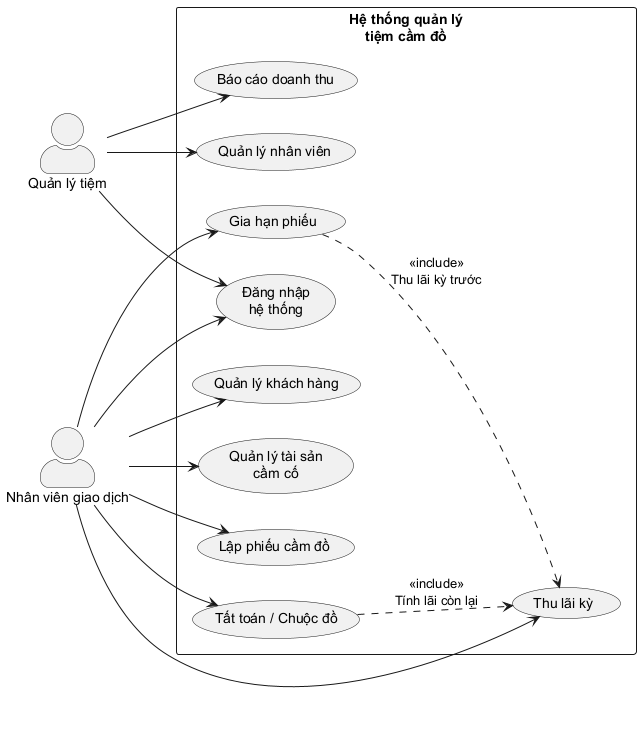
\includegraphics[width=\textwidth]{diagrams/pawnshop_usecase_overall.png}
  \caption{Use Case tổng quan hệ thống quản lý tiệm cầm đồ}
  \label{fig:uc_overall}
\end{figure}

\section{Use Case phân rã nghiệp vụ phiếu cầm}

Để nhìn rõ hơn mối quan hệ giữa các chức năng trong vòng đời một phiếu cầm đồ, hình~\ref{fig:uc_pawn_flow} mô tả Use Case phân rã xung quanh tác nhân ``Nhân viên giao dịch''. Use Case trung tâm là ``Quản lý phiếu cầm đồ'', bao gồm bốn Use Case con chính: lập phiếu cầm, thu lãi kỳ, gia hạn phiếu và tất toán/chuộc đồ. Các Use Case mở rộng như thanh toán lãi qua mã QR, thanh toán tất toán qua QR và in phiếu được mô hình hóa dưới dạng \emph{extend} để nhấn mạnh rằng chúng không bắt buộc xảy ra trong mọi lần thực hiện nghiệp vụ nhưng thường xuyên được sử dụng trong thực tế.

\begin{figure}[H]
  \centering
  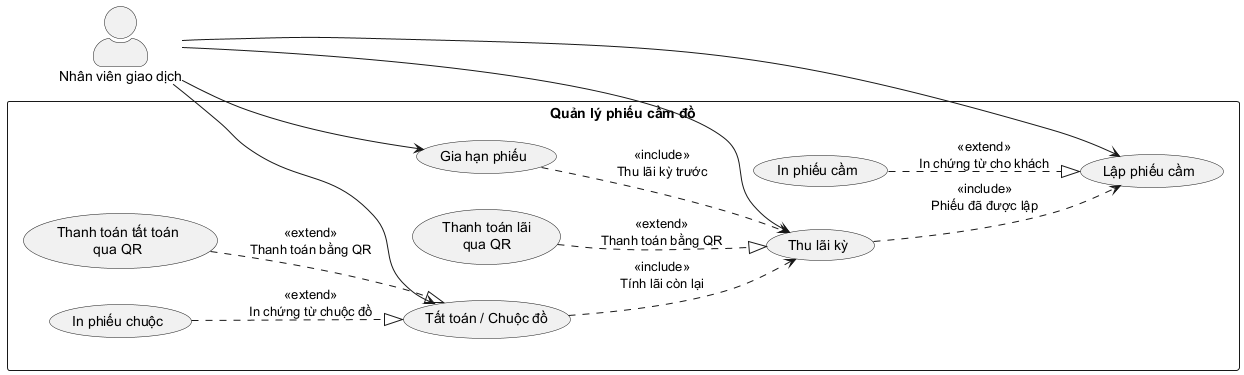
\includegraphics[width=\textwidth]{diagrams/pawnshop_usecase_pawn_flow.png}
  \caption{Use Case phân rã nghiệp vụ quản lý phiếu cầm đồ}
  \label{fig:uc_pawn_flow}
\end{figure}

Trong sơ đồ này, Use Case ``Thu lãi kỳ'' \emph{include} Use Case ``Lập phiếu cầm'' vì mọi hoạt động thu lãi đều phải gắn với một phiếu đã được lập trước đó. Use Case ``Gia hạn phiếu'' \emph{include} ``Thu lãi kỳ'' để thể hiện quy tắc nghiệp vụ: trước khi tăng thêm số ngày cầm, hệ thống luôn thu lãi kỳ trước. Tương tự, Use Case ``Tất toán/Chuộc đồ'' \emph{include} việc tính lãi còn lại trên phiếu. Các Use Case ``Thanh toán lãi qua QR'' và ``Thanh toán tất toán qua QR'' được thể hiện dưới dạng \emph{extend} của ``Thu lãi kỳ'' và ``Tất toán/Chuộc đồ'', cho thấy đây là các kịch bản tùy chọn bổ sung, chỉ được kích hoạt khi khách lựa chọn hình thức thanh toán chuyển khoản.

\section{Use Case phân rã nghiệp vụ khách hàng}

Bên cạnh nghiệp vụ phiếu cầm, nghiệp vụ quản lý khách hàng cũng giữ vai trò quan trọng vì là điểm xuất phát của hầu hết các giao dịch trong tiệm. Hình~\ref{fig:uc_customers} mô tả Use Case phân rã cho chức năng ``Quản lý khách hàng'' với các Use Case con: thêm khách hàng mới, cập nhật thông tin khách hàng và tra cứu khách hàng. Trong đó, ``Cập nhật thông tin khách hàng'' và ``Tra cứu khách hàng'' đều \emph{include} ``Thêm khách hàng mới'' theo nghĩa logic: mọi thao tác tra cứu hoặc chỉnh sửa đều dựa trên dữ liệu khách hàng đã được thêm vào hệ thống trước đó.

\begin{figure}[H]
  \centering
  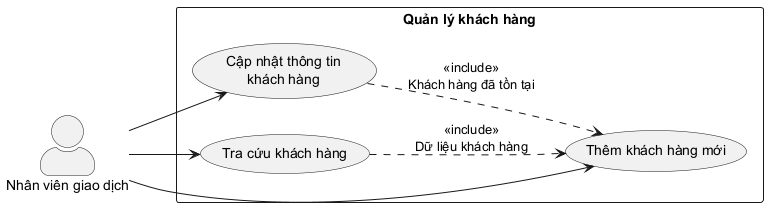
\includegraphics[width=\textwidth]{diagrams/pawnshop_usecase_customers.png}
  \caption{Use Case phân rã nghiệp vụ quản lý khách hàng}
  \label{fig:uc_customers}
\end{figure}

Use Case ``Thêm khách hàng mới'' mô tả việc ghi nhận lần đầu tiên thông tin một khách hàng đến tiệm, bao gồm họ tên, số điện thoại, CMND/CCCD và địa chỉ. Use Case ``Cập nhật thông tin khách hàng'' cho phép chỉnh sửa thông tin này khi khách có thay đổi về địa chỉ, số điện thoại hoặc giấy tờ tùy thân. Use Case ``Tra cứu khách hàng'' được sử dụng thường xuyên khi nhân viên cần lập phiếu cầm mới cho khách cũ hoặc xem lại lịch sử giao dịch; việc tra cứu có thể dựa trên tên, số điện thoại hoặc số CMND/CCCD, giúp giảm thiểu việc tạo trùng nhiều hồ sơ cho cùng một khách hàng.

\section{Sơ đồ chức năng (BFD)}

Để mô tả cách hệ thống được phân rã thành các nhóm chức năng nghiệp vụ, khóa luận sử dụng sơ đồ chức năng kinh doanh (BFD). Ở mức 0, hệ thống được xem như một khối chức năng lớn có nhiệm vụ quản lý toàn bộ hoạt động của tiệm cầm đồ. Hình~\ref{fig:bfd0} trình bày các chức năng chính: quản lý khách hàng, quản lý tài sản cầm cố, quản lý phiếu cầm đồ, quản lý thu lãi/gia hạn/tất toán, quản lý báo cáo và quản lý nhân viên.

\begin{figure}[H]
  \centering
  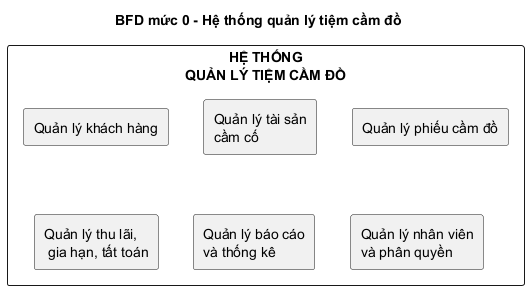
\includegraphics[width=\textwidth]{diagrams/pawnshop_bfd_level0.png}
  \caption{BFD mức 0 – Chức năng tổng quát của hệ thống}
  \label{fig:bfd0}
\end{figure}

BFD mức 1 (hình~\ref{fig:bfd1}) đi sâu hơn vào chức năng ``Quản lý phiếu cầm đồ'', tách thành các chức năng con như quản lý thông tin phiếu cầm, quản lý lịch sử thu lãi và gia hạn, quản lý tất toán và trạng thái phiếu. Cách phân rã này giúp làm rõ ràng phạm vi trách nhiệm của từng nhóm chức năng, thuận tiện cho việc phân công nhiệm vụ khi triển khai và bảo trì hệ thống.

\begin{figure}[H]
  \centering
  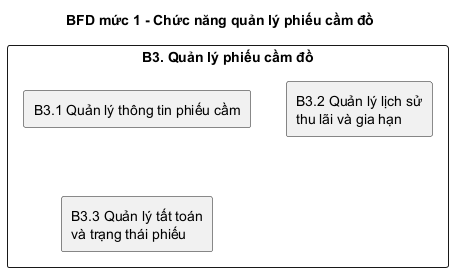
\includegraphics[width=0.7\textwidth]{diagrams/pawnshop_bfd_level1.png}
  \caption{BFD mức 1 – Phân rã chức năng quản lý phiếu cầm đồ}
  \label{fig:bfd1}
\end{figure}

Ở mức 2, khóa luận tập trung vào chức năng ``Quản lý lịch sử thu lãi và gia hạn''. Hình~\ref{fig:bfd2} cho thấy chức năng này tiếp tục được chia thành các chức năng nhỏ hơn như tính lãi đến thời điểm hiện tại, ghi nhận thu lãi kỳ, ghi nhận gia hạn phiếu và cập nhật ngày tính lãi tiếp theo. Việc phân rã đến mức 2 giúp việc hiện thực và kiểm thử từng phần trở nên dễ dàng, đồng thời bảo đảm rằng khảo sát nghiệp vụ đã bao quát đầy đủ các bước xử lý quan trọng trong thực tế.

\begin{figure}[H]
  \centering
  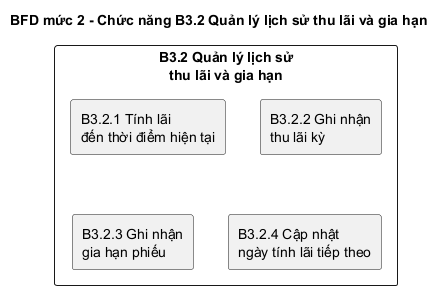
\includegraphics[width=0.7\textwidth]{diagrams/pawnshop_bfd_level2.png}
  \caption{BFD mức 2 – Phân rã chức năng quản lý lịch sử thu lãi và gia hạn}
  \label{fig:bfd2}
\end{figure}

\section{Đặc tả một số Use Case chính}

\subsection*{Đăng nhập hệ thống}

\begin{table}[H]
\centering
\caption{Đặc tả Use Case: Đăng nhập hệ thống}
\label{tab:uc-login}
\begin{tabular}{p{4cm}p{10cm}}
\hline
Tên Use Case & Đăng nhập hệ thống\\
\hline
Tác nhân chính & Quản lý tiệm, Nhân viên giao dịch\\
Mục tiêu & Xác thực tài khoản người dùng trước khi cho phép truy cập các chức năng quản lý.\\
Tiền điều kiện & Tài khoản đã được tạo và đang ở trạng thái hoạt động.\\
Kết quả & Người dùng đăng nhập thành công và được chuyển đến màn hình Dashboard.\\
\hline
Luồng sự kiện chính &
\begin{enumerate}
\item Người dùng truy cập trang \texttt{/login} và nhập tên đăng nhập, mật khẩu.
\item Hệ thống kiểm tra thông tin nhập vào, tìm kiếm người dùng tương ứng trong cơ sở dữ liệu.
\item Nếu thông tin hợp lệ và tài khoản đang hoạt động, Flask-Login tạo phiên làm việc và lưu thông tin người dùng vào session.
\item Hệ thống chuyển hướng người dùng tới trang Dashboard.
\end{enumerate}\\
\hline
Luồng ngoại lệ &
Nếu tên đăng nhập hoặc mật khẩu không chính xác, hoặc tài khoản đã bị khóa, hệ thống hiển thị thông báo lỗi ``Sai tên đăng nhập hoặc mật khẩu'' và giữ nguyên tại trang đăng nhập.\\
\hline
\end{tabular}
\end{table}

\subsection*{Lập phiếu cầm đồ}

\begin{table}[H]
\centering
\caption{Đặc tả Use Case: Lập phiếu cầm đồ}
\label{tab:uc-pawn}
\begin{tabular}{p{4cm}p{10cm}}
\hline
Tên Use Case & Lập phiếu cầm đồ\\
\hline
Tác nhân chính & Nhân viên giao dịch\\
Mục tiêu & Ghi nhận thông tin khách hàng, tài sản và khoản tiền cầm trong một phiếu cầm hợp lệ.\\
Tiền điều kiện & Nhân viên đã đăng nhập; khách hàng đã có trong hệ thống hoặc được thêm mới.\\
Kết quả & Phiếu cầm được tạo, sinh mã phiếu, lưu lại lịch sử và chuyển sang trạng thái ``Đang cầm''.\\
\hline
Luồng sự kiện chính &
\begin{enumerate}
  \item Nhân viên chọn khách hàng từ danh sách hoặc tạo mới khách hàng.
  \item Nhân viên nhập thông tin tài sản cầm (tên, loại, giá trị ước tính) và số tiền cầm.
  \item Nhân viên điều chỉnh lãi suất, số ngày cầm nếu cần, đồng thời có thể nhập thông tin người mang tài sản đến tiệm nếu khác với chủ sở hữu.
  \item Hệ thống sinh mã phiếu theo cấu trúc ngày--số thứ tự, tính hạn chuộc dựa trên số ngày cầm và lưu phiếu vào cơ sở dữ liệu.
  \item Hệ thống chuyển hướng nhân viên tới trang chi tiết phiếu để theo dõi lãi và in phiếu cho khách hàng ký.
\end{enumerate}\\
\hline
Luồng ngoại lệ &
Nếu thiếu thông tin bắt buộc (khách hàng, tên tài sản, số tiền cầm) hoặc số tiền cầm không hợp lệ, hệ thống hiển thị thông báo lỗi và không lưu phiếu.\\
\hline
\end{tabular}
\end{table}

\subsection*{Tất toán / Chuộc đồ}

\begin{table}[H]
\centering
\caption{Đặc tả Use Case: Tất toán / Chuộc đồ}
\label{tab:uc-redeem}
\begin{tabular}{p{4cm}p{10cm}}
\hline
Tên Use Case & Tất toán / Chuộc đồ\\
\hline
Tác nhân chính & Nhân viên giao dịch\\
Mục tiêu & Tính toán số tiền khách cần thanh toán để chuộc tài sản và cập nhật trạng thái phiếu sang ``Đã chuộc''.\\
Tiền điều kiện & Phiếu đang ở trạng thái ``Đang cầm'', ``Đã gia hạn'' hoặc ``Quá hạn''.\\
Kết quả & Trạng thái phiếu chuyển sang ``Đã chuộc'', tạo bản ghi thu tiền tương ứng.\\
\hline
Luồng sự kiện chính &
\begin{enumerate}
  \item Nhân viên mở trang chi tiết phiếu và chọn chức năng ``Tất toán / Chuộc đồ'' hoặc ``QR tất toán''.
  \item Hệ thống tính lãi còn lại từ lần thu lãi/gia hạn gần nhất đến ngày hiện tại, cộng với tiền gốc để ra tổng tiền phải thu.
  \item Nếu khách thanh toán bằng tiền mặt, nhân viên xác nhận đã nhận đủ tiền; nếu khách thanh toán qua QR, hệ thống sinh mã QR VietQR với nội dung và số tiền tương ứng để khách quét chuyển khoản.
  \item Sau khi thanh toán thành công, hệ thống lưu bản ghi \texttt{Payment} loại ``redeem'', cập nhật trường \texttt{redeem\_amount}, \texttt{redeem\_date} và chuyển trạng thái phiếu sang ``Đã chuộc''.
\end{enumerate}\\
\hline
Luồng ngoại lệ &
Nếu trong quá trình tính toán phát hiện phiếu đã ở trạng thái ``Đã chuộc'' hoặc số tiền cần thanh toán bằng không, hệ thống hiển thị thông báo và không thực hiện tất toán lần nữa.\\
\hline
\end{tabular}
\end{table}

\subsection*{Gia hạn phiếu cầm đồ}

\begin{table}[H]
\centering
\caption{Đặc tả Use Case: Gia hạn phiếu cầm đồ}
\label{tab:uc-extend}
\begin{tabular}{p{4cm}p{10cm}}
\hline
Tên Use Case & Gia hạn phiếu cầm đồ\\
\hline
Tác nhân chính & Nhân viên giao dịch\\
Mục tiêu & Cho phép khách hàng tiếp tục cầm tài sản sau khi đã thanh toán lãi kỳ trước.\\
Tiền điều kiện & Phiếu đang ở trạng thái ``Đang cầm'' hoặc ``Đã gia hạn'' và chưa quá hạn.\\
Kết quả & Hạn chuộc được dời thêm số ngày gia hạn, lãi kỳ trước được ghi nhận.\\
\hline
Luồng sự kiện chính &
\begin{enumerate}
  \item Nhân viên mở trang chi tiết phiếu và nhấn nút ``Gia hạn''.
  \item Hệ thống hiển thị form cho phép nhập số ngày gia hạn mong muốn.
  \item Nhân viên nhập số ngày gia hạn và xác nhận.
  \item Hệ thống tính lãi kỳ trước, tạo bản ghi \texttt{Payment} loại ``extension'' và cộng thêm số ngày gia hạn vào hạn chuộc.
  \item Hệ thống cập nhật lại thông tin phiếu và hiển thị hạn chuộc mới trong màn hình chi tiết.
\end{enumerate}\\
\hline
Luồng ngoại lệ &
Nếu phiếu đã quá hạn hoặc số lần gia hạn vượt quá giới hạn cho phép, hệ thống hiển thị thông báo lỗi và không thực hiện gia hạn.\\
\hline
\end{tabular}
\end{table}

\subsection*{Quản lý khách hàng}

\begin{table}[H]
\centering
\caption{Đặc tả Use Case: Quản lý khách hàng}
\label{tab:uc-customers}
\begin{tabular}{p{4cm}p{10cm}}
\hline
Tên Use Case & Quản lý khách hàng\\
\hline
Tác nhân chính & Nhân viên giao dịch, Quản lý tiệm\\
Mục tiêu & Lưu trữ và tra cứu thông tin khách hàng phục vụ cho việc lập và tra cứu phiếu cầm.\\
Tiền điều kiện & Người dùng đã đăng nhập hệ thống.\\
Kết quả & Thông tin khách hàng được thêm mới, chỉnh sửa hoặc xem chi tiết theo yêu cầu.\\
\hline
Luồng sự kiện chính &
\begin{enumerate}
  \item Người dùng truy cập màn hình ``Khách hàng'' từ menu điều hướng.
  \item Hệ thống hiển thị danh sách khách hàng kèm các trường cơ bản như họ tên, số điện thoại, CMND/CCCD.
  \item Khi cần thêm mới, người dùng nhấn nút ``Thêm khách hàng'', nhập thông tin và bấm lưu.
  \item Khi cần chỉnh sửa, người dùng chọn một dòng trong bảng, nhấn ``Sửa'' và cập nhật lại thông tin cần thiết.
  \item Khi cần tra cứu, người dùng sử dụng ô tìm kiếm theo tên hoặc số điện thoại, hệ thống lọc danh sách tương ứng.
\end{enumerate}\\
\hline
Luồng ngoại lệ &
Nếu người dùng nhập trùng số CMND/CCCD hoặc số điện thoại đã tồn tại, hệ thống hiển thị thông báo lỗi và yêu cầu kiểm tra lại thông tin.\\
\hline
\end{tabular}
\end{table}

\subsection*{Báo cáo doanh thu}

\begin{table}[H]
\centering
\caption{Đặc tả Use Case: Báo cáo doanh thu}
\label{tab:uc-reports}
\begin{tabular}{p{4cm}p{10cm}}
\hline
Tên Use Case & Báo cáo doanh thu\\
\hline
Tác nhân chính & Quản lý tiệm\\
Mục tiêu & Tổng hợp doanh thu gốc và lãi theo khoảng thời gian để đánh giá hiệu quả hoạt động của tiệm.\\
Tiền điều kiện & Người dùng đăng nhập với vai trò quản lý.\\
Kết quả & Hệ thống hiển thị biểu đồ và bảng số liệu doanh thu theo tháng trong năm được chọn.\\
\hline
Luồng sự kiện chính &
\begin{enumerate}
  \item Quản lý truy cập màn hình ``Báo cáo''.
  \item Người dùng chọn năm cần xem báo cáo, nhấn nút ``Xem''.
  \item Hệ thống truy vấn bảng \texttt{transactions} và \texttt{payments}, tính tổng tiền gốc đã chuộc và tổng tiền lãi đã thu cho từng tháng.
  \item Kết quả được biểu diễn dưới dạng biểu đồ cột và bảng chi tiết bên dưới.
  \item Quản lý có thể dựa vào số liệu để so sánh hoạt động giữa các tháng và đưa ra quyết định điều chỉnh phù hợp.
\end{enumerate}\\
\hline
Luồng ngoại lệ &
Nếu trong năm được chọn chưa có dữ liệu, hệ thống hiển thị thông báo ``Chưa có dữ liệu để báo cáo'' và không vẽ biểu đồ.\\
\hline
\end{tabular}
\end{table}

\subsection*{Quản lý nhân viên}

\begin{table}[H]
\centering
\caption{Đặc tả Use Case: Quản lý nhân viên}
\label{tab:uc-users}
\begin{tabular}{p{4cm}p{10cm}}
\hline
Tên Use Case & Quản lý nhân viên\\
\hline
Tác nhân chính & Quản lý tiệm\\
Mục tiêu & Tạo, chỉnh sửa và khóa/mở tài khoản nhân viên để kiểm soát quyền truy cập hệ thống.\\
Tiền điều kiện & Người dùng đăng nhập với vai trò quản lý.\\
Kết quả & Danh sách tài khoản nhân viên được cập nhật đúng với tình hình nhân sự thực tế.\\
\hline
Luồng sự kiện chính &
\begin{enumerate}
  \item Quản lý truy cập màn hình ``Nhân viên''.
  \item Hệ thống hiển thị danh sách tài khoản nhân viên kèm tên đăng nhập, họ tên, vai trò và trạng thái.
  \item Khi cần tạo mới, quản lý nhấn nút ``Thêm nhân viên'', nhập thông tin cần thiết và lưu lại.
  \item Khi cần khóa hoặc mở khóa tài khoản, quản lý nhấn nút tương ứng trên dòng nhân viên, hệ thống cập nhật trạng thái \texttt{is\_active}.
  \item Khi cần đặt lại mật khẩu, quản lý sử dụng chức năng ``Reset mật khẩu'' để hệ thống sinh mật khẩu mới và thông báo cho nhân viên.
\end{enumerate}\\
\hline
Luồng ngoại lệ &
Nếu quản lý cố gắng khóa tài khoản của chính mình hoặc tài khoản quản trị duy nhất, hệ thống từ chối thao tác và hiển thị thông báo cảnh báo.\\
\hline
\end{tabular}
\end{table}

\section{Mô hình dữ liệu và sơ đồ lớp}

\begin{figure}[H]
  \centering
  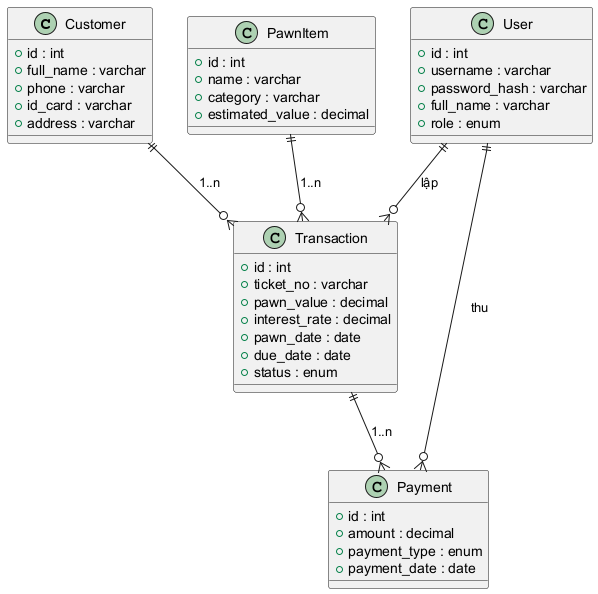
\includegraphics[width=\textwidth]{diagrams/pawnshop_erd.png}
  \caption{Sơ đồ ERD hệ thống quản lý tiệm cầm đồ}
  \label{fig:erd}
\end{figure}

\begin{figure}[H]
  \centering
  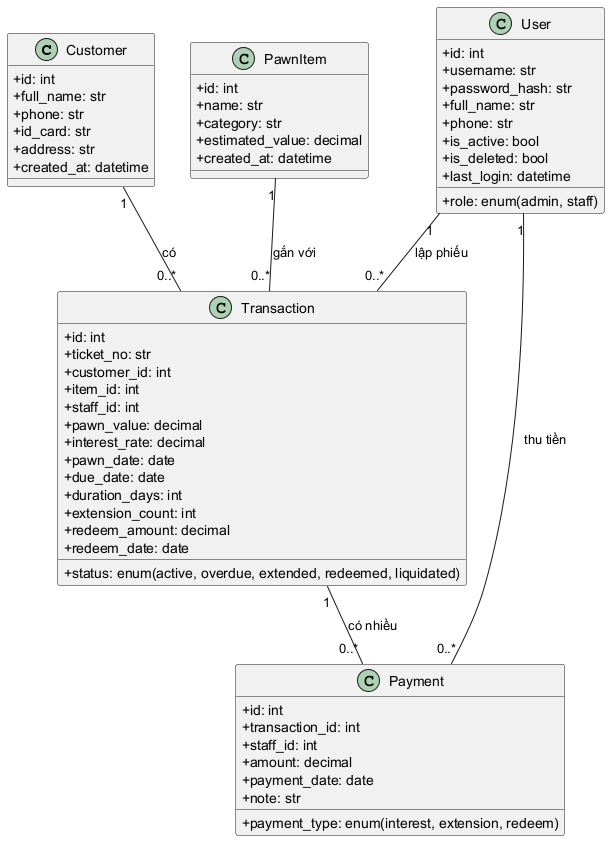
\includegraphics[width=\textwidth]{diagrams/pawnshop_class_model.png}
  \caption{Sơ đồ lớp các thực thể chính của hệ thống}
  \label{fig:class_domain}
\end{figure}

Sơ đồ ERD ở hình~\ref{fig:erd} mô tả các bảng chính trong cơ sở dữ liệu và mối quan hệ giữa chúng. Thực thể \texttt{Customer} liên kết một-nhiều với \texttt{Transaction}, phản ánh việc mỗi khách hàng có thể có nhiều phiếu cầm tại tiệm. Thực thể \texttt{PawnItem} cũng liên kết một-nhiều với \texttt{Transaction}, cho phép một loại tài sản có thể được sử dụng lại trong nhiều phiếu cầm khác nhau theo thời gian. Bảng \texttt{Transaction} liên kết một-nhiều với \texttt{Payment}, thể hiện lịch sử các lần thu lãi, gia hạn và tất toán cho từng phiếu. Thực thể \texttt{User} liên kết với cả \texttt{Transaction} và \texttt{Payment}, ghi nhận nhân viên chịu trách nhiệm lập phiếu và thu tiền.

Sơ đồ lớp ở hình~\ref{fig:class_domain} chi tiết hóa các thuộc tính và mối quan hệ này ở mức độ hướng đối tượng trong mã nguồn Python. Các lớp \texttt{Customer}, \texttt{PawnItem}, \texttt{Transaction}, \texttt{Payment}, \texttt{User} tương ứng với các bảng trong cơ sở dữ liệu, nhưng được bổ sung thêm các thuộc tính và phương thức phục vụ logic nghiệp vụ như tính trạng thái phiếu, xác định lần thu lãi gần nhất hoặc định dạng thông tin hiển thị trên giao diện. Việc duy trì sự tương ứng chặt chẽ giữa ERD và sơ đồ lớp giúp quá trình triển khai bằng SQLAlchemy trở nên rõ ràng, đồng thời giảm khả năng xảy ra sai lệch giữa thiết kế và hiện thực.

\section{Sơ đồ luồng dữ liệu (DFD)}

Song song với BFD và ERD, sơ đồ luồng dữ liệu (DFD) cung cấp một góc nhìn khác về hệ thống, tập trung vào các tiến trình xử lý, luồng dữ liệu và kho dữ liệu. DFD mức 0 (hình~\ref{fig:dfd0}) mô tả hệ thống quản lý tiệm cầm đồ như một tiến trình duy nhất, tương tác với ba tác nhân bên ngoài là khách hàng, nhân viên giao dịch và quản lý tiệm. Các luồng dữ liệu chính bao gồm thông tin khách hàng, yêu cầu cầm đồ, thông tin phiếu, phiếu thu, phiếu chuộc và báo cáo doanh thu.

\begin{figure}[H]
  \centering
  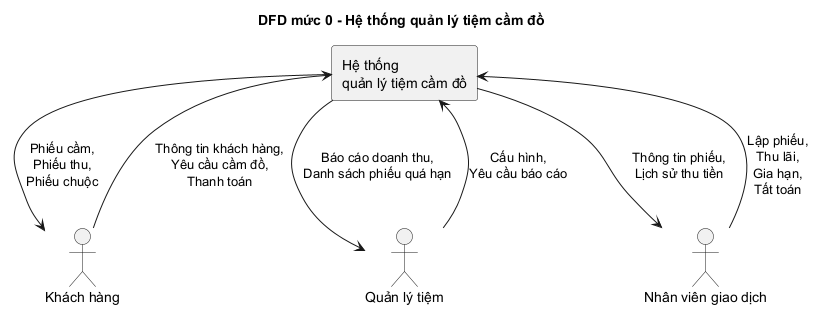
\includegraphics[width=\textwidth]{diagrams/pawnshop_dfd_level0.png}
  \caption{DFD mức 0 – Hệ thống quản lý tiệm cầm đồ}
  \label{fig:dfd0}
\end{figure}

DFD mức 1 (hình~\ref{fig:dfd1}) phân rã hệ thống thành năm tiến trình chính: quản lý khách hàng, quản lý tài sản, quản lý phiếu cầm, quản lý thu lãi/gia hạn/tất toán và lập báo cáo doanh thu. Các kho dữ liệu tương ứng là danh sách khách hàng, danh sách tài sản, danh sách phiếu cầm và danh sách bản ghi thu tiền. Sơ đồ cho thấy rõ mối liên hệ giữa các tiến trình: kết quả của tiến trình quản lý phiếu cầm và quản lý thu lãi được sử dụng làm đầu vào cho tiến trình lập báo cáo, trong khi tiến trình quản lý khách hàng và tài sản cung cấp dữ liệu nền cho toàn bộ hệ thống.

\begin{figure}[H]
  \centering
  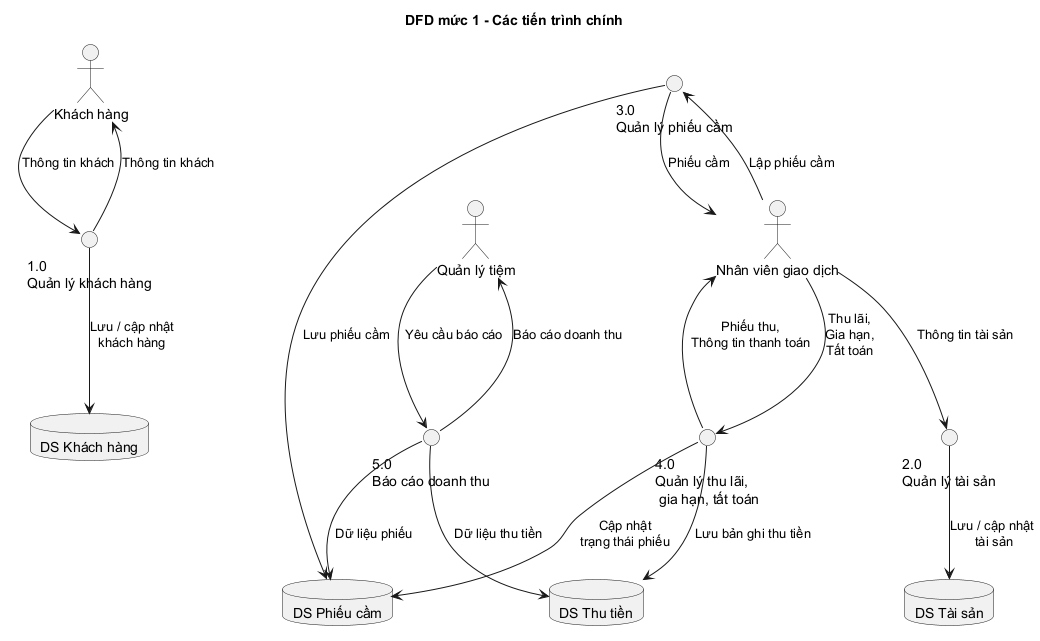
\includegraphics[width=\textwidth]{diagrams/pawnshop_dfd_level1.png}
  \caption{DFD mức 1 – Các tiến trình chính và kho dữ liệu}
  \label{fig:dfd1}
\end{figure}

Đối với tiến trình 3.0 ``Quản lý phiếu cầm'', DFD mức 2 (hình~\ref{fig:dfd2}) đi sâu vào ba tiến trình con: tiếp nhận yêu cầu cầm đồ, lập phiếu cầm và cập nhật thông tin phiếu cầm. Nhân viên giao dịch cung cấp thông tin khách hàng và tài sản cho tiến trình tiếp nhận yêu cầu; tiến trình này có thể truy vấn hoặc cập nhật kho dữ liệu khách hàng và tài sản trước khi chuyển thông tin đã kiểm tra sang tiến trình lập phiếu cầm. Sau khi phiếu được lập, dữ liệu được lưu vào kho phiếu cầm và được trả ngược lại cho nhân viên dưới dạng mã phiếu và nội dung phiếu. Khi có yêu cầu chỉnh sửa phiếu, tiến trình cập nhật thông tin phiếu cầm sẽ truy vấn và cập nhật lại kho dữ liệu tương ứng. Việc phân rã đến mức này giúp nhóm dễ dàng đối chiếu giữa yêu cầu nghiệp vụ, thiết kế và quá trình hiện thực mã nguồn.

\begin{figure}[H]
  \centering
  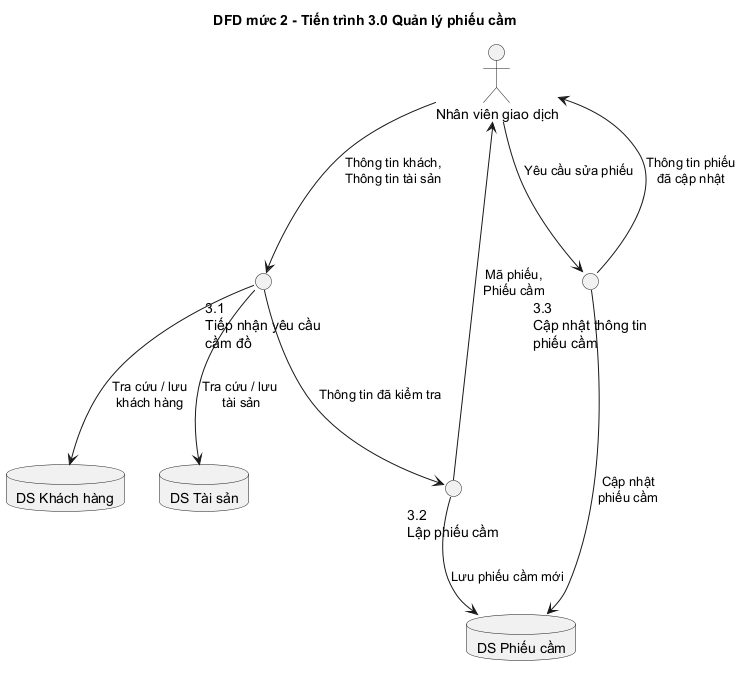
\includegraphics[width=\textwidth]{diagrams/pawnshop_dfd_level2_pawn.png}
  \caption{DFD mức 2 – Tiến trình 3.0 Quản lý phiếu cầm}
  \label{fig:dfd2}
\end{figure}

%---------------------------------------
\chapter{THIẾT KẾ GIAO DIỆN VÀ KIẾN TRÚC}
%---------------------------------------

\section{Kiến trúc dự án}

Hệ thống quản lý tiệm cầm đồ được tổ chức theo kiến trúc một ứng dụng Flask duy nhất, chia thành các lớp logic rõ ràng. Lớp giao diện người dùng bao gồm các template Jinja2 trong thư mục \texttt{app/views}, được xây dựng dựa trên hai layout chính là \texttt{layouts/base.html} cho phần backend và \texttt{layouts/auth.html} cho trang đăng nhập. Lớp điều khiển gồm các blueprint \texttt{auth}, \texttt{dashboard}, \texttt{transactions}, \texttt{customers}, \texttt{items}, \texttt{reports}, \texttt{users}, mỗi blueprint chịu trách nhiệm cho một nhóm chức năng cụ thể. Lớp dữ liệu bao gồm các model SQLAlchemy được định nghĩa trong \texttt{app/models}, kết nối tới cơ sở dữ liệu MySQL thông qua cấu hình tập trung trong \texttt{config.py}.

Giữa các lớp này, dữ liệu được truyền dưới dạng đối tượng và dictionary, hạn chế truy cập trực tiếp tới cơ sở dữ liệu từ template. Các controller xử lý logic nghiệp vụ như tính lãi, xác định lần thu lãi gần nhất, gia hạn phiếu, tất toán phiếu, sinh mã phiếu, đồng thời ghi nhận lịch sử thu tiền vào bảng \texttt{payments}. Một số logic tính toán chuyên biệt được tách ra khỏi controller dưới dạng service, tiêu biểu là \texttt{app.services.interest.calc\_interest} dùng để tính lãi dựa trên số tiền cầm, lãi suất tháng và số ngày; \texttt{app.services.vietqr.build\_qr\_url} dùng để xây dựng đường dẫn mã QR VietQR cho thanh toán chuyển khoản.

\section{Một số màn hình chính của hệ thống}

\begin{figure}[H]
  \centering
  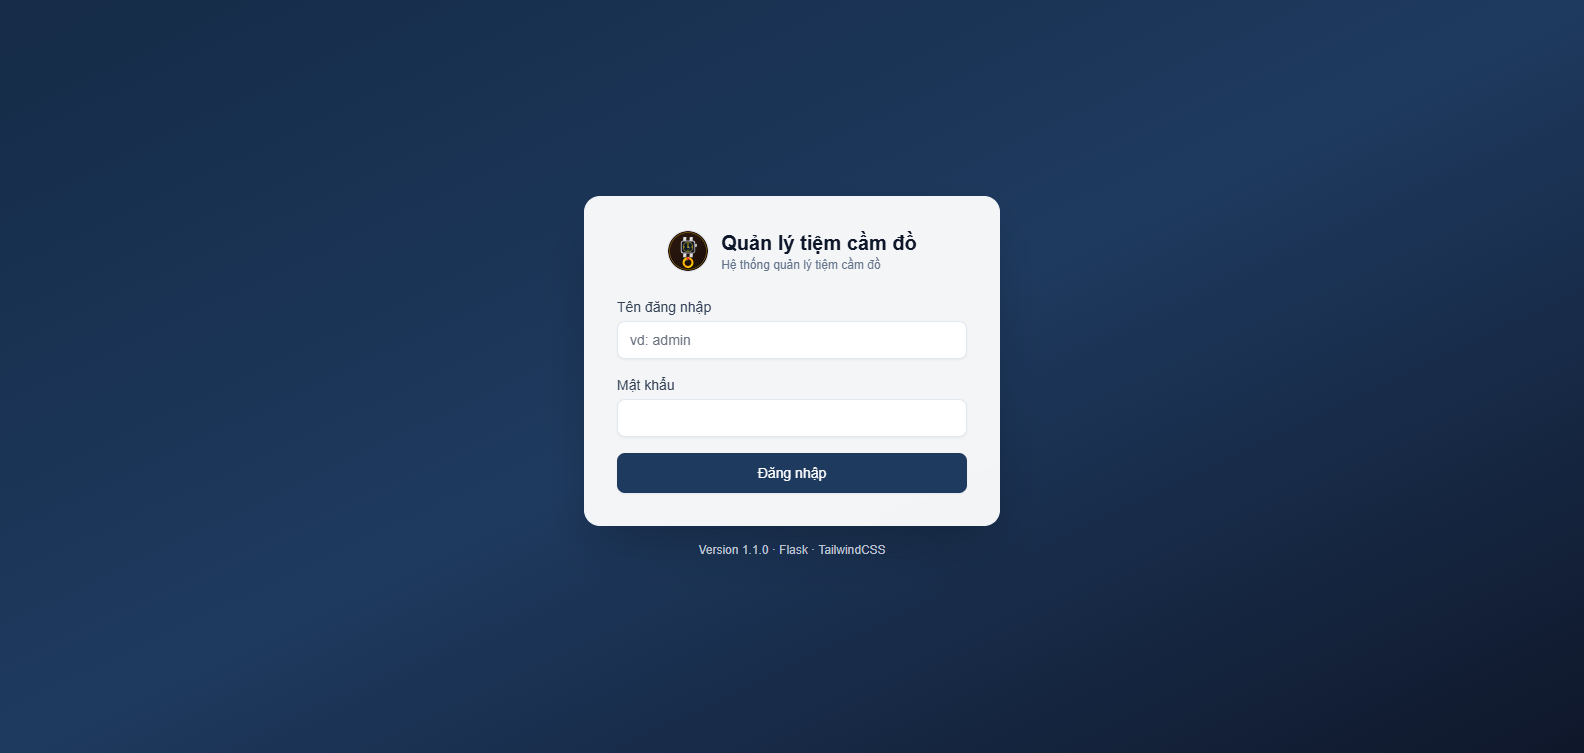
\includegraphics[width=\textwidth]{screenshots_admin/00_login.png}
  \caption{Giao diện đăng nhập hệ thống quản lý tiệm cầm đồ}
  \label{fig:login}
\end{figure}




\begin{figure}[H]
  \centering
  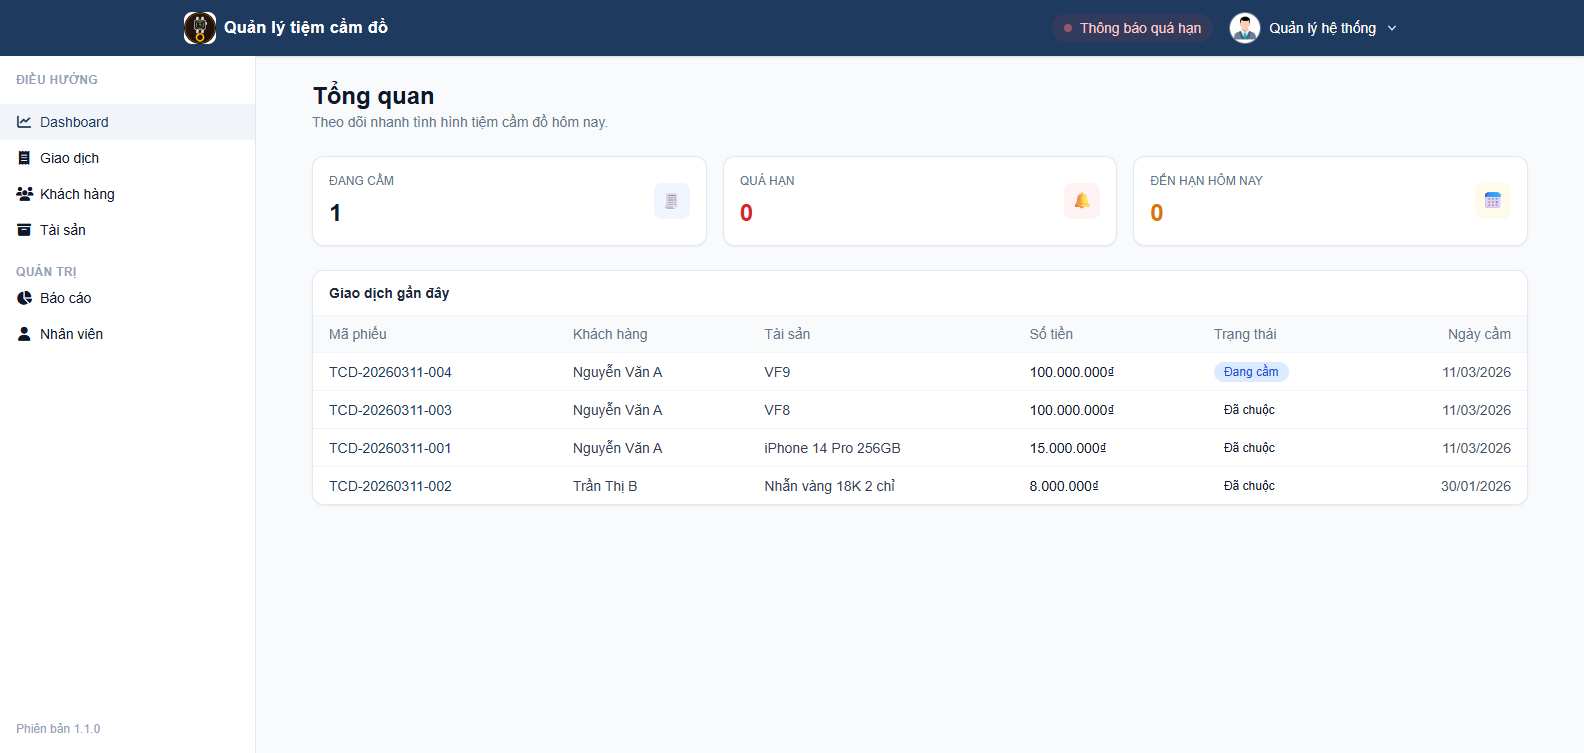
\includegraphics[width=\textwidth]{screenshots_admin/01_dashboard.png}
  \caption{Màn hình Dashboard theo dõi nhanh tình hình tiệm}
  \label{fig:dashboard}
\end{figure}

\begin{figure}[H]
  \centering
  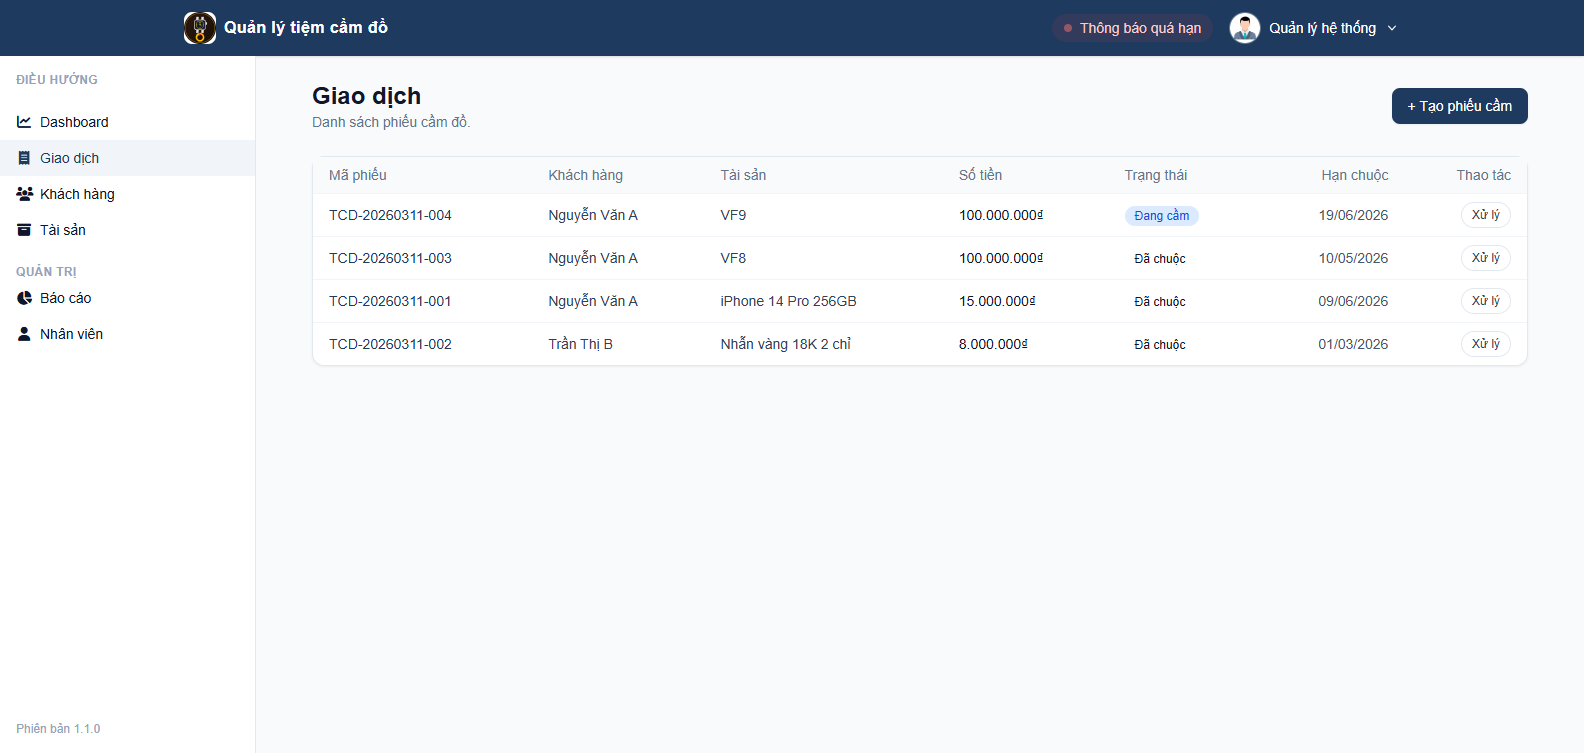
\includegraphics[width=\textwidth]{screenshots_admin/02_transactions_list.png}
  \caption{Danh sách phiếu cầm đồ trong hệ thống}
  \label{fig:transactions_list}
\end{figure}

\begin{figure}[H]
  \centering
  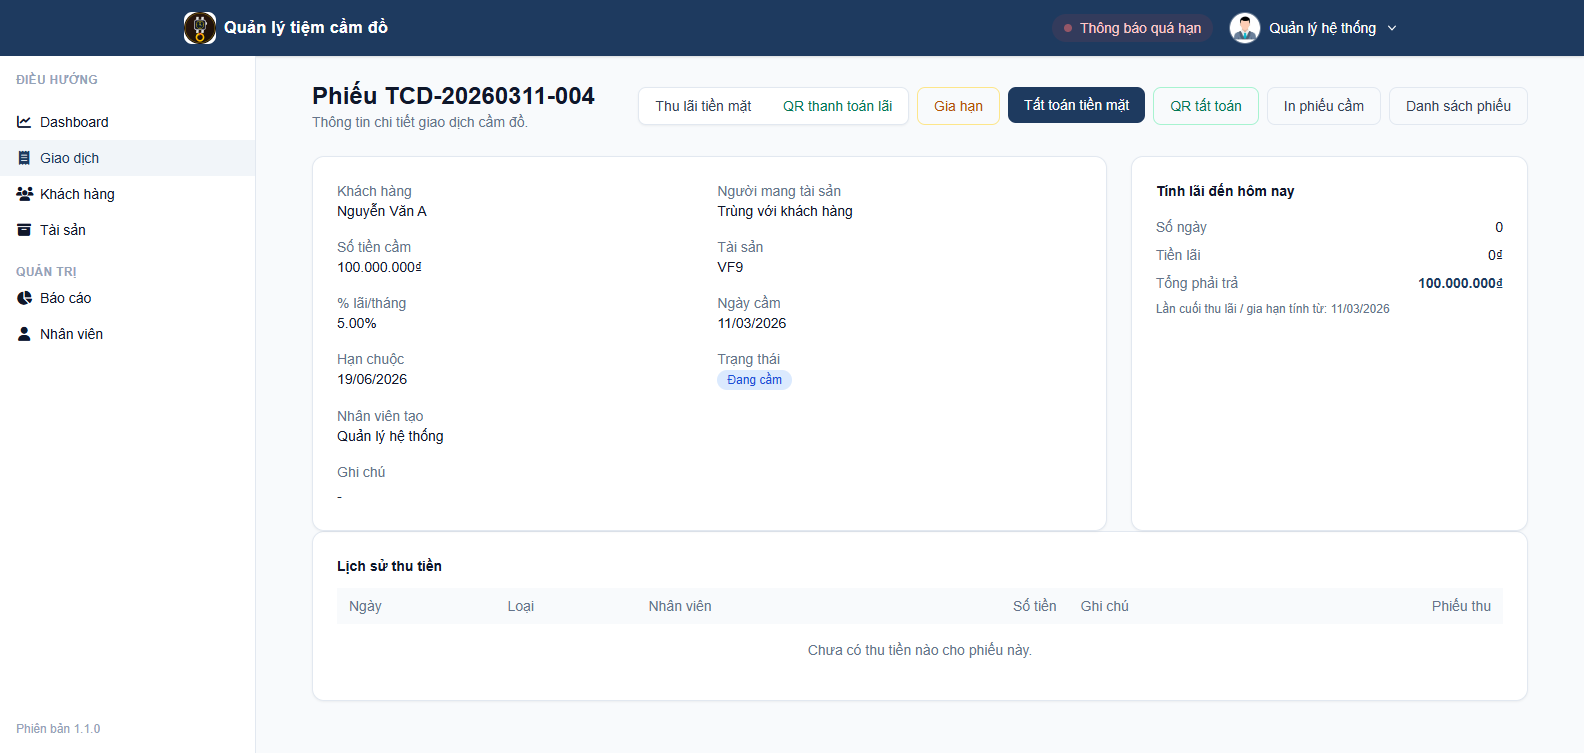
\includegraphics[width=\textwidth]{screenshots_admin/03_transaction_detail.png}
  \caption{Chi tiết một phiếu cầm đồ}
  \label{fig:transaction_detail}
\end{figure}

\begin{figure}[H]
  \centering
  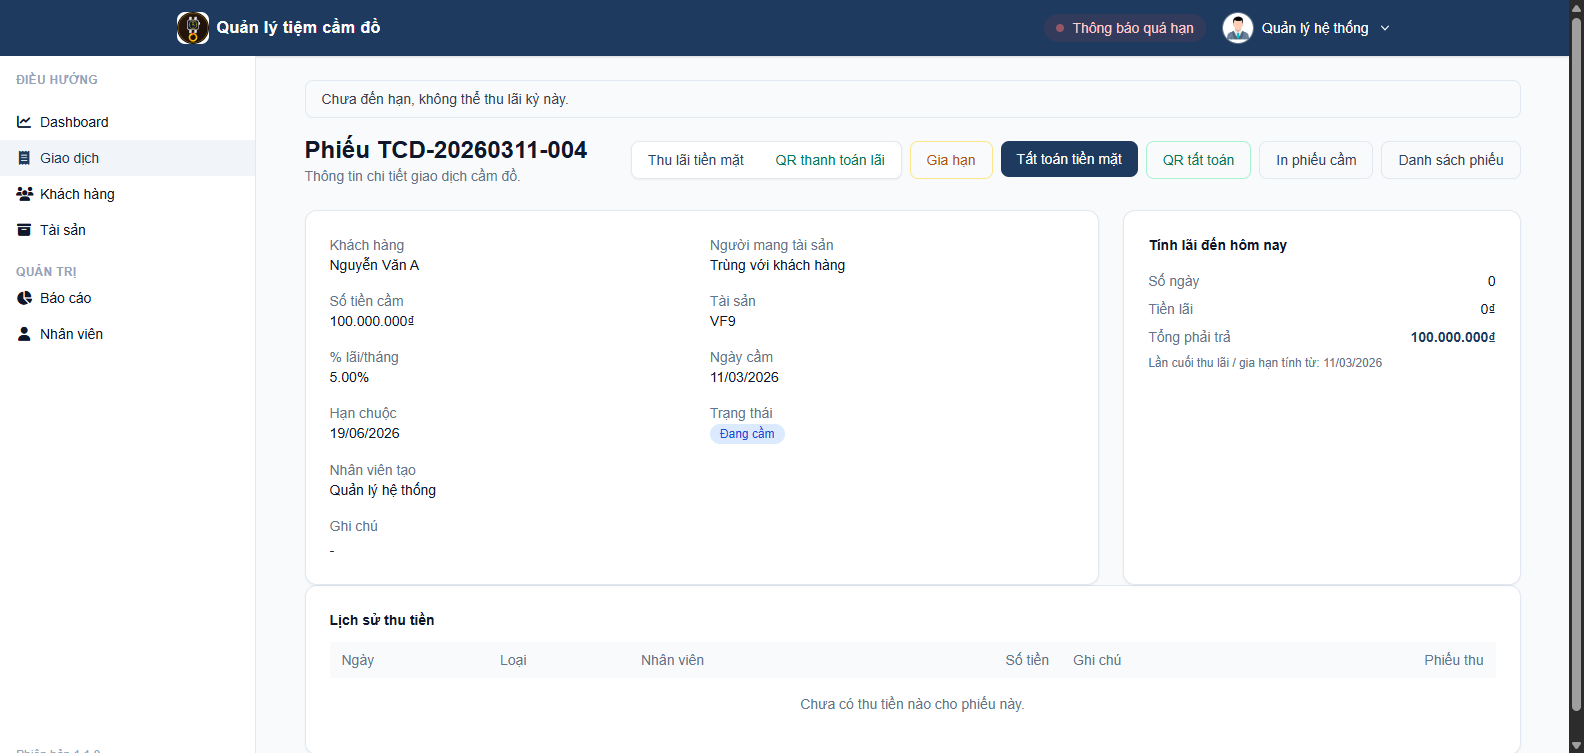
\includegraphics[width=\textwidth]{screenshots_admin/10_qr_interest.png}
  \caption{Thanh toán lãi qua mã QR ngân hàng}
  \label{fig:qr_interest}
\end{figure}

\begin{figure}[H]
  \centering
  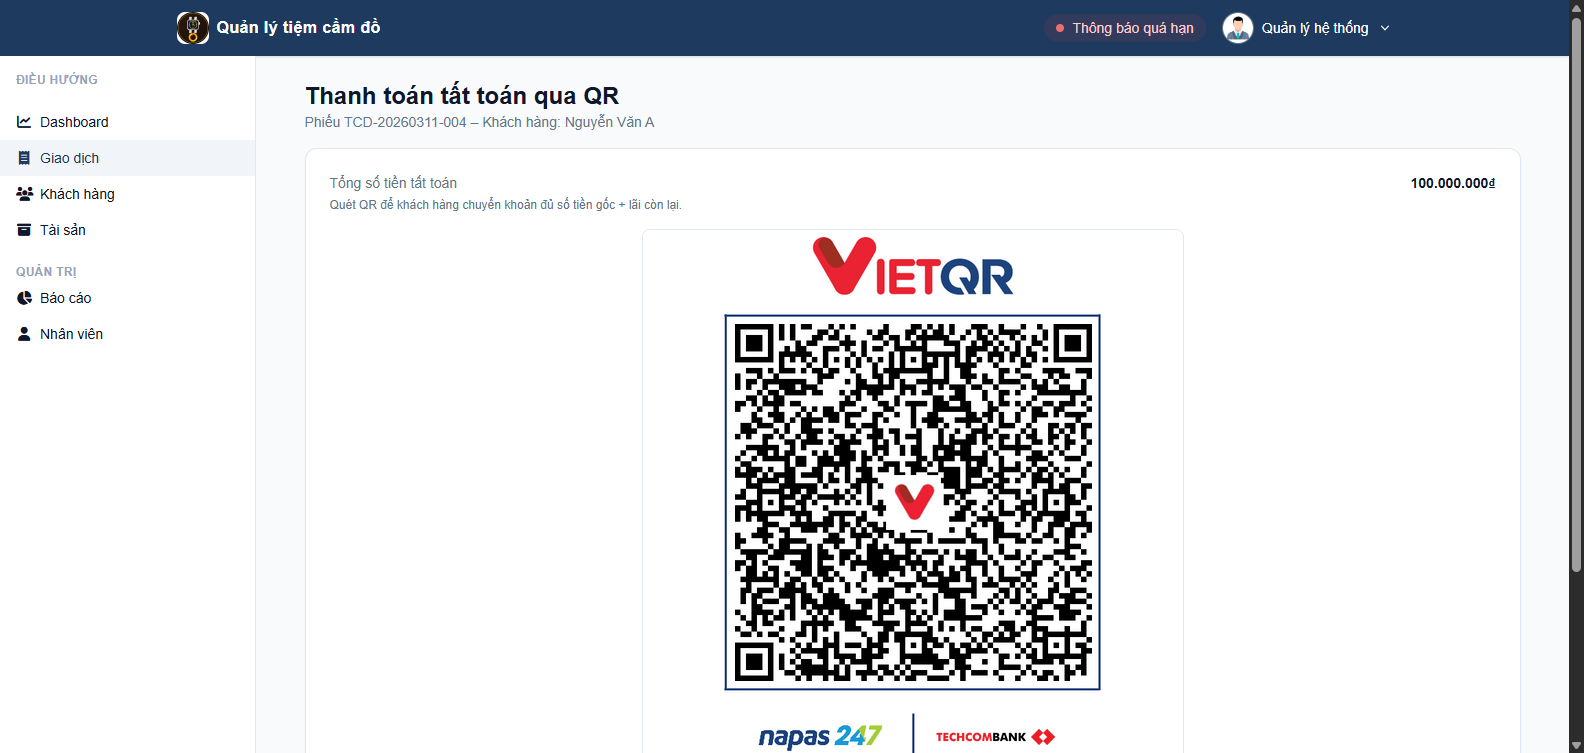
\includegraphics[width=\textwidth]{screenshots_admin/11_qr_redeem.png}
  \caption{Thanh toán tất toán phiếu cầm qua QR}
  \label{fig:qr_redeem}
\end{figure}

\begin{figure}[H]
  \centering
  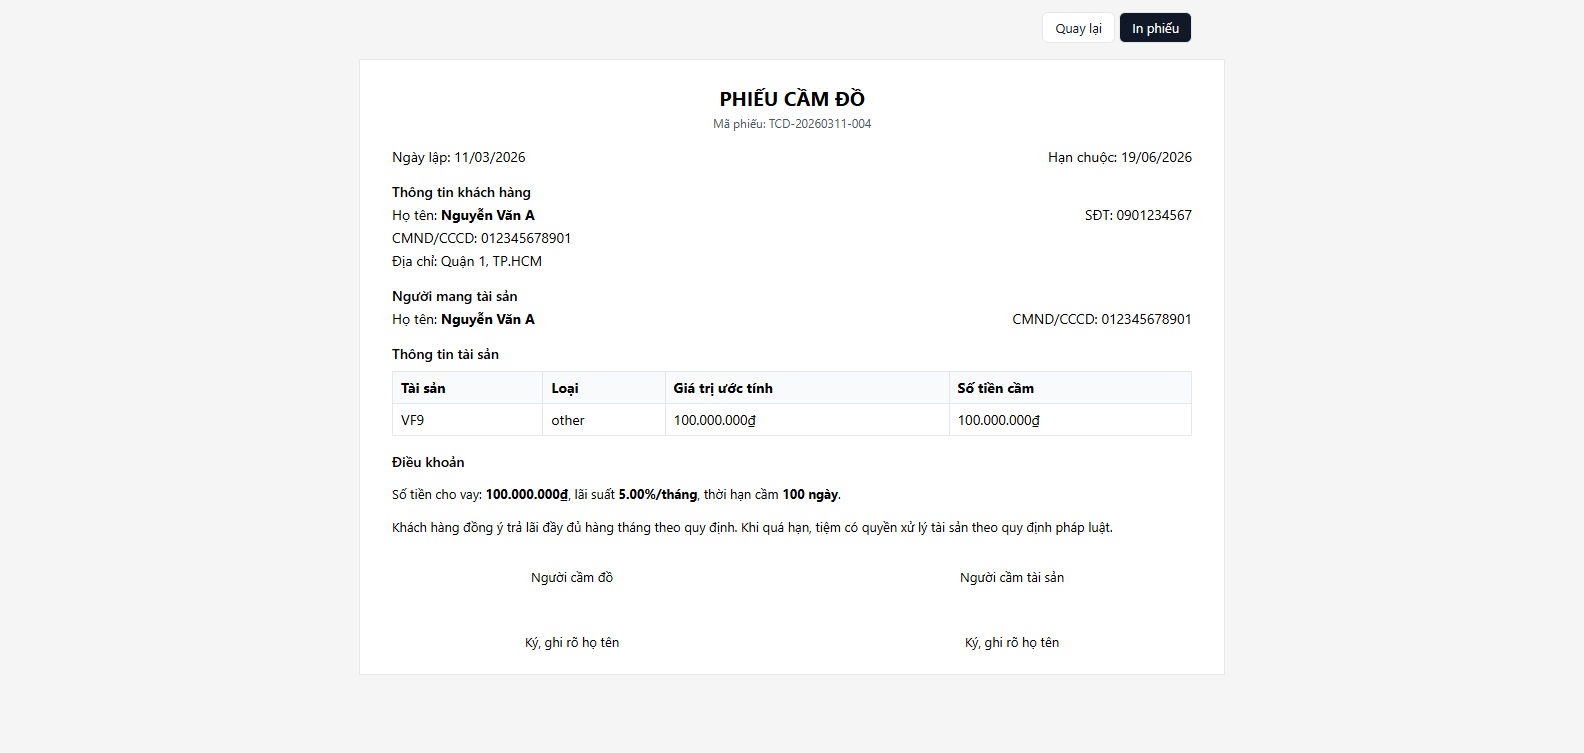
\includegraphics[width=\textwidth]{screenshots_admin/12_print_ticket.png}
  \caption{Mẫu phiếu cầm đồ được in từ hệ thống}
  \label{fig:print_ticket}
\end{figure}

\begin{figure}[H]
  \centering
  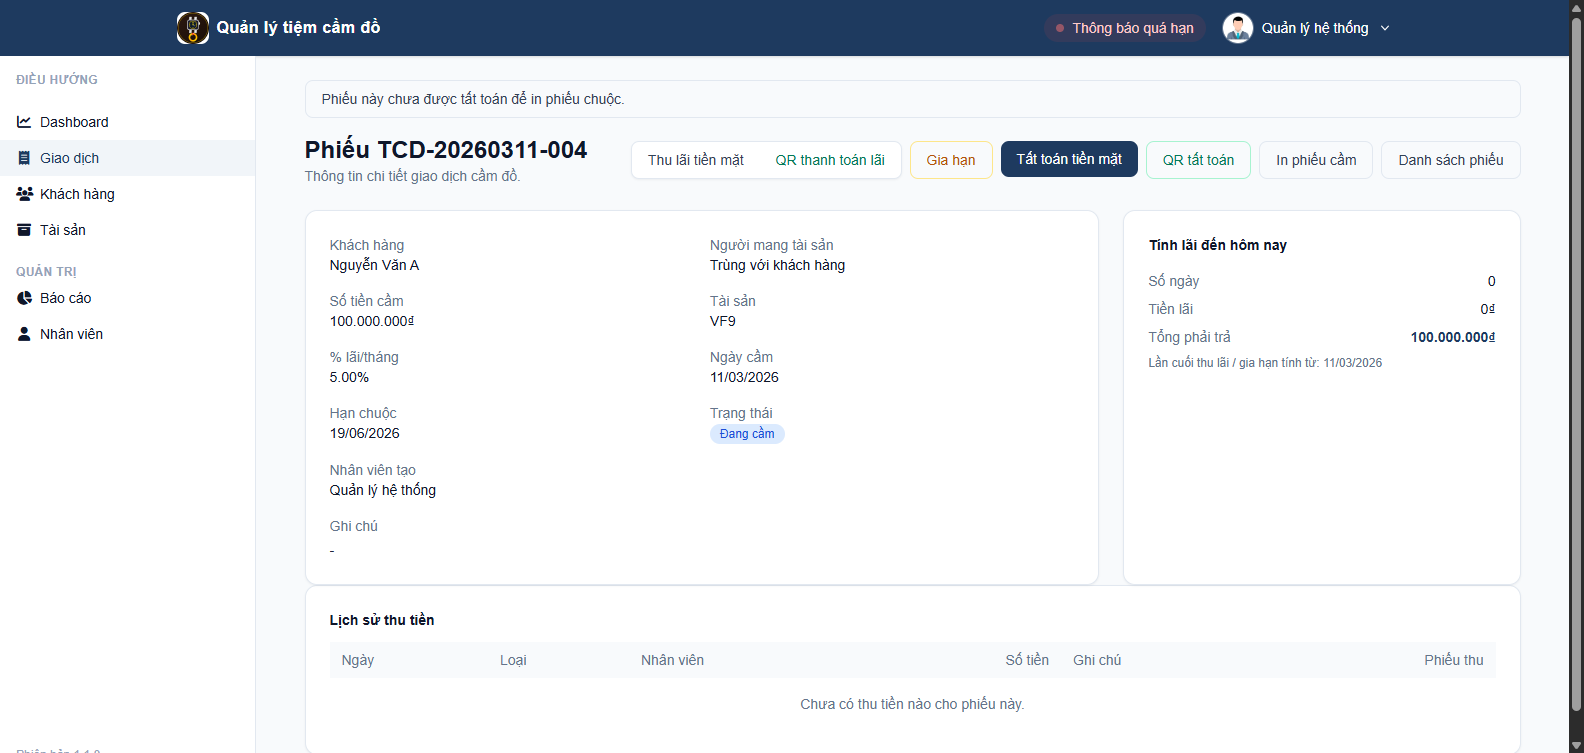
\includegraphics[width=\textwidth]{screenshots_admin/13_print_redeem.png}
  \caption{Mẫu phiếu chuộc đồ được in từ hệ thống}
  \label{fig:print_redeem}
\end{figure}

\begin{figure}[H]
  \centering
  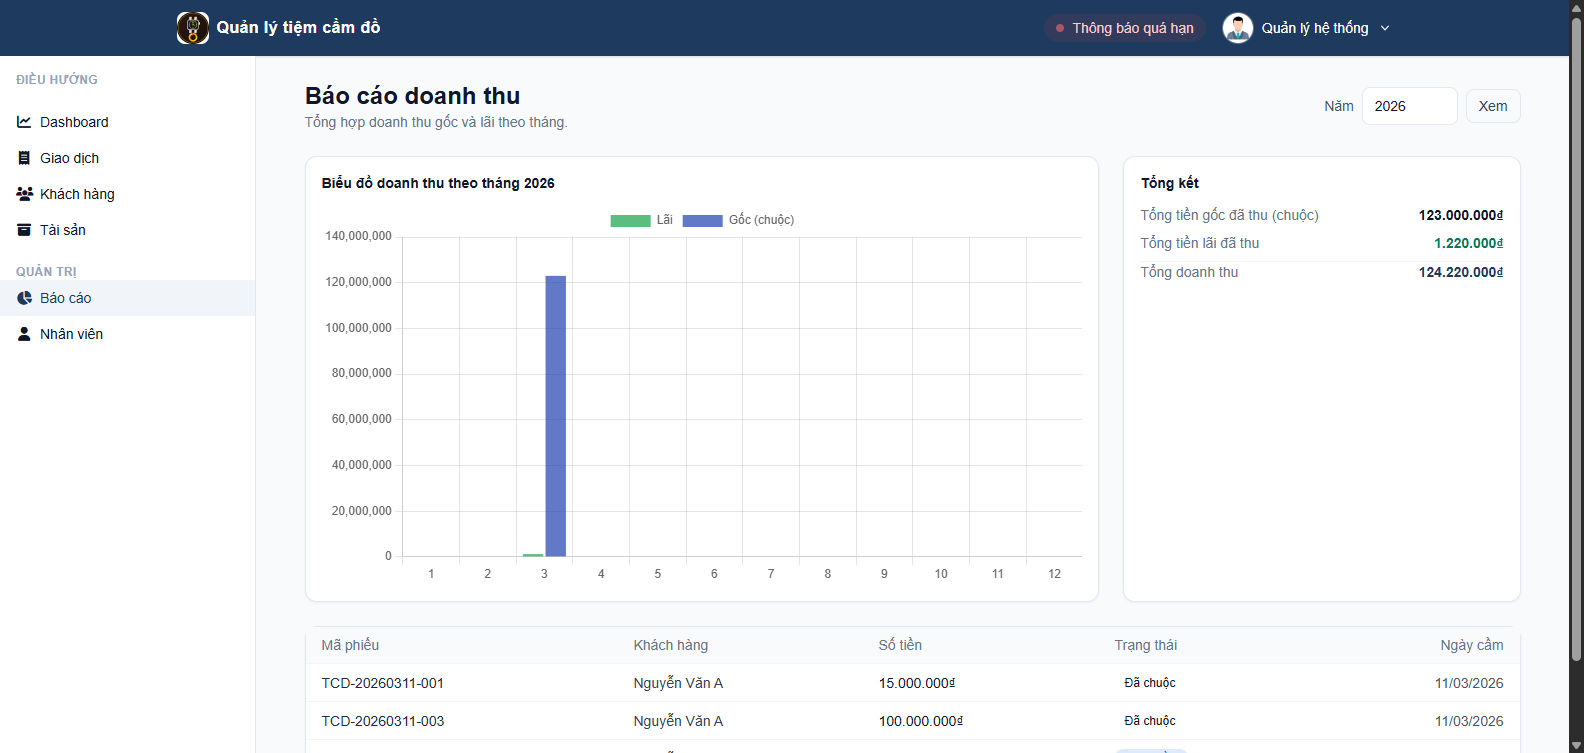
\includegraphics[width=\textwidth]{screenshots_admin/07_reports.png}
  \caption{Màn hình báo cáo doanh thu gốc và lãi}
  \label{fig:reports}
\end{figure}

\section{Thiết kế giao diện theo từng phân hệ}

Giao diện người dùng của hệ thống được thiết kế xoay quanh một layout thống nhất gồm thanh tiêu đề phía trên, thanh điều hướng bên trái và vùng nội dung chính ở giữa. Thanh điều hướng hiển thị các nhóm chức năng ``Dashboard'', ``Giao dịch'', ``Khách hàng'', ``Tài sản'', ``Báo cáo'' và ``Nhân viên'' dưới dạng danh sách, mỗi mục tương ứng với một blueprint trong Flask. Khi người dùng chọn một mục bất kỳ, phần nội dung được nạp lại nhưng khung xương layout vẫn giữ nguyên, giúp trải nghiệm sử dụng mạch lạc và nhất quán.

Ở phân hệ giao dịch, màn hình danh sách phiếu cầm tập trung vào việc cung cấp cho nhân viên cái nhìn nhanh về các phiếu hiện có, với các cột thông tin quan trọng như mã phiếu, khách hàng, tài sản, số tiền cầm, trạng thái và hạn chuộc. Các trạng thái được hiển thị dưới dạng badge màu để dễ nhận biết: màu xanh cho ``Đang cầm'', vàng cho ``Đã gia hạn'', đỏ cho ``Quá hạn'' và xanh lá cho ``Đã chuộc''. Khi người dùng chọn một phiếu, hệ thống chuyển tới màn hình chi tiết phiếu, nơi tập trung các nút thao tác chính như thu lãi, gia hạn, tất toán, thanh toán QR và in phiếu.

Phân hệ khách hàng được tổ chức theo dạng bảng với ô tìm kiếm ở phía trên, cho phép lọc theo tên hoặc số điện thoại. Khi nhấn vào tên một khách hàng, người dùng được chuyển tới màn hình chi tiết khách hàng, nơi hiển thị đầy đủ thông tin cá nhân và lịch sử các phiếu cầm mà khách đã tham gia. Cách trình bày này giúp nhân viên nhanh chóng nắm được mối quan hệ giữa khách hàng và các phiếu cầm, thuận tiện cho việc tư vấn hoặc xử lý khi khách quay lại giao dịch.

Phân hệ báo cáo được thiết kế theo hướng trực quan, lấy năm làm tham số chính để lọc dữ liệu. Sau khi người dùng chọn năm và nhấn nút xem, biểu đồ cột thể hiện doanh thu gốc và lãi theo từng tháng được hiển thị ở phần giữa, bên cạnh một bảng số liệu chi tiết. Phần bên phải là vùng tổng kết, hiển thị tổng tiền gốc đã chuộc, tổng tiền lãi đã thu và tổng doanh thu trong năm. Cách bố trí này giúp quản lý vừa có cái nhìn tổng thể qua biểu đồ, vừa có thể đối chiếu nhanh với số liệu cụ thể trong bảng.

Cuối cùng, phân hệ quản lý nhân viên cung cấp danh sách tài khoản dưới dạng bảng với các thông tin như tên đăng nhập, họ tên, vai trò, trạng thái hoạt động và các nút chức năng như khóa/mở, đặt lại mật khẩu. Giao diện được xây dựng đơn giản nhưng rõ ràng, giúp quản lý dễ dàng thao tác trên các tài khoản, đồng thời nhờ thiết kế badge màu cho trạng thái hoạt động mà có thể nhanh chóng nhận diện những tài khoản đang bị khóa hay đã xóa mềm.

\section{Sơ đồ triển khai hệ thống}

\begin{figure}[H]
  \centering
  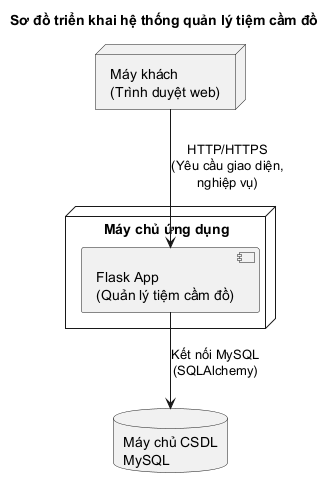
\includegraphics[width=0.8\textwidth]{diagrams/pawnshop_deployment.png}
  \caption{Sơ đồ triển khai hệ thống quản lý tiệm cầm đồ}
  \label{fig:deployment}
\end{figure}

%---------------------------------------
\chapter{XÂY DỰNG HỆ THỐNG}
%---------------------------------------

Chương này trình bày chi tiết cách nhóm hiện thực hệ thống quản lý tiệm cầm đồ trên nền tảng Flask, bao gồm tổ chức dự án, các module chính và cách triển khai những nghiệp vụ quan trọng như lập phiếu cầm, thu lãi, gia hạn, tất toán, in phiếu và thanh toán qua mã QR.

\section{Cấu trúc dự án và tổ chức thư mục}

Mã nguồn hệ thống được tổ chức trong thư mục \texttt{app} theo phong cách ``blueprint'' của Flask. Các thư mục con quan trọng bao gồm \texttt{models} (chứa các lớp ánh xạ cơ sở dữ liệu), \texttt{controllers} (chứa các blueprint xử lý nghiệp vụ), \texttt{views} (chứa các template Jinja2) và \texttt{services} (chứa các hàm tính toán, tiện ích dùng chung). Tập tin \texttt{config.py} định nghĩa các thông số cấu hình như chuỗi kết nối MySQL, số dòng phân trang, lãi suất mặc định và các tham số cho dịch vụ VietQR.

Trong nhóm model, lớp \texttt{Customer} lưu trữ thông tin khách hàng và được liên kết một-nhiều với \texttt{Transaction}. Lớp \texttt{PawnItem} mô tả tài sản cầm cố, tách rời khỏi khách hàng để tiện tái sử dụng trong trường hợp khách cầm nhiều lần cùng một loại tài sản. Lớp \texttt{Transaction} thể hiện phiếu cầm với các trường như mã phiếu, khách hàng, tài sản, nhân viên lập phiếu, số tiền cầm, lãi suất, ngày cầm, hạn chuộc, số lần gia hạn và trạng thái. Lớp \texttt{Payment} ghi nhận từng lần thu tiền, phân biệt rõ các loại giao dịch ``interest'', ``extension'' và ``redeem'', làm nền tảng cho module báo cáo doanh thu. Cuối cùng, lớp \texttt{User} mô tả tài khoản nhân viên với các thuộc tính phục vụ phân quyền như \texttt{role}, \texttt{is\_active}, \texttt{is\_deleted}.

\section{Mô hình kiến trúc Flask theo MVC}

Xét về mặt kiến trúc, hệ thống quản lý tiệm cầm đồ bám khá sát mô hình MVC (Model--View--Controller) quen thuộc trong các ứng dụng web. ``Model'' trong hệ thống được hiện thực bởi các lớp SQLAlchemy trong thư mục \texttt{app/models}, chịu trách nhiệm ánh xạ dữ liệu giữa đối tượng Python và bảng MySQL. ``View'' được đảm nhiệm bởi các template Jinja2 trong \texttt{app/views}, nơi định nghĩa cấu trúc HTML và cách hiển thị dữ liệu cho người dùng cuối. ``Controller'' tương ứng với các blueprint trong \texttt{app/controllers}, là nơi tiếp nhận HTTP request, gọi model và service để xử lý nghiệp vụ rồi lựa chọn template phù hợp để render.

Hình~\ref{fig:architecture} mô tả mối quan hệ giữa các thành phần chính trong kiến trúc này. Ở phía trình duyệt, người dùng tương tác với giao diện HTML được kết hợp với TailwindCSS để định dạng. Các yêu cầu từ trình duyệt được gửi đến các blueprint như \texttt{auth}, \texttt{dashboard}, \texttt{transactions}, \texttt{customers}, \texttt{items}, \texttt{reports}, \texttt{users}. Mỗi blueprint đóng vai trò như một nhóm controller chuyên trách cho một phân hệ: \texttt{transactions} xử lý toàn bộ nghiệp vụ phiếu cầm, từ lập phiếu, thu lãi, gia hạn đến tất toán; \texttt{customers} xử lý nghiệp vụ khách hàng; \texttt{reports} chịu trách nhiệm tính toán dữ liệu báo cáo dựa trên bảng \texttt{transactions} và \texttt{payments}.

Bên dưới tầng controller là các model và service. Các lớp \texttt{Customer}, \texttt{PawnItem}, \texttt{Transaction}, \texttt{Payment}, \texttt{User} chứa logic liên quan trực tiếp đến dữ liệu như ràng buộc khóa ngoại, mối quan hệ giữa các bảng và một số thuộc tính tính toán đơn giản. Những nghiệp vụ phức tạp hơn như tính lãi theo ngày hoặc sinh đường dẫn mã QR được tách ra thành các service độc lập trong \texttt{app/services} (\texttt{interest.calc\_interest}, \texttt{vietqr.build\_qr\_url}). Điều này giúp controller nhẹ hơn, dễ kiểm thử và dễ mở rộng khi cần bổ sung thêm nghiệp vụ mà không làm rối mã nguồn.

Ở tầng thấp nhất, toàn bộ model thông qua SQLAlchemy tương tác với cơ sở dữ liệu MySQL. Kiến trúc này cho phép việc thay đổi giao diện (View) hoặc thay đổi một phần nghiệp vụ ở controller không ảnh hưởng trực tiếp tới cấu trúc dữ liệu bên dưới, đồng thời vẫn giữ được mối liên hệ chặt chẽ giữa ba phần Model--View--Controller.

\begin{figure}[H]
  \centering
  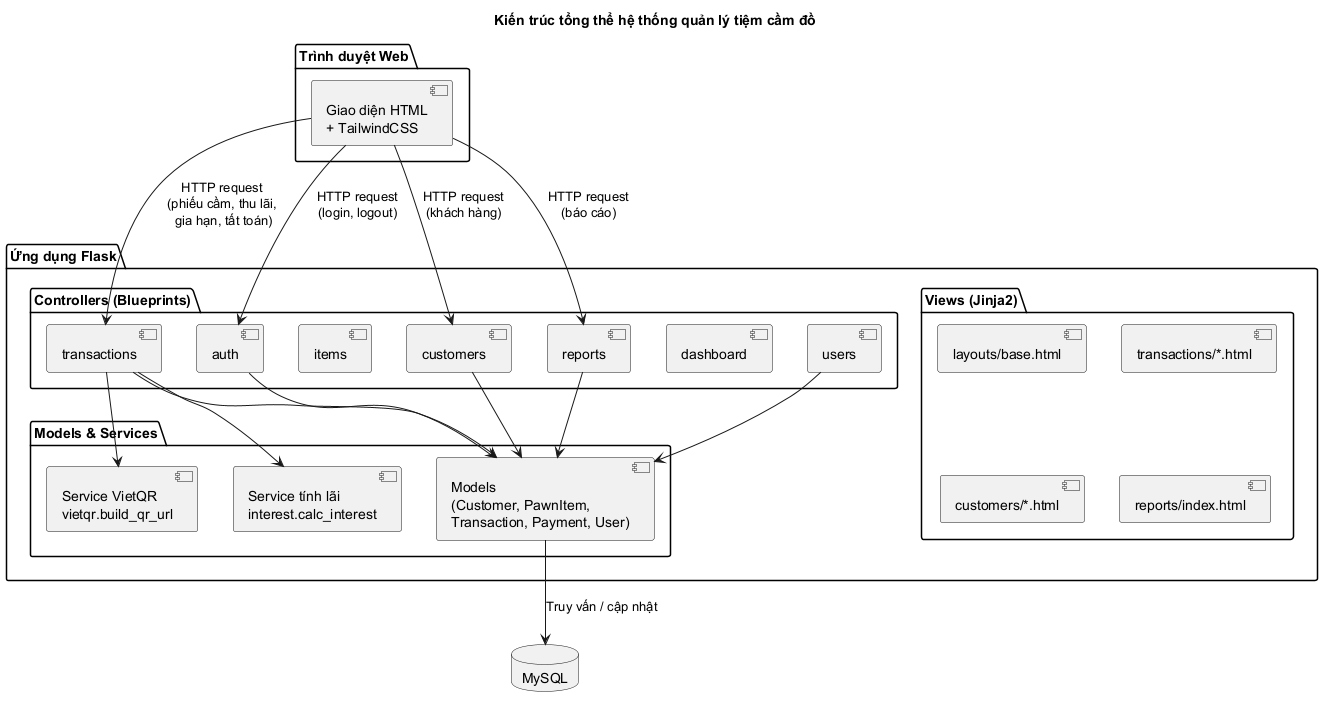
\includegraphics[width=\textwidth]{diagrams/pawnshop_architecture.png}
  \caption{Kiến trúc tổng thể hệ thống theo mô hình Flask MVC}
  \label{fig:architecture}
\end{figure}

\section{Hiện thực các nghiệp vụ cốt lõi}

Các nghiệp vụ chính của tiệm cầm đồ được hiện thực chủ yếu trong blueprint \texttt{transactions}. Khi người dùng truy cập trang tạo phiếu, hệ thống tải danh sách khách hàng để nhân viên lựa chọn, đồng thời cho phép nhập thông tin người mang tài sản và tài sản cầm. Sau khi nhân viên nhập số tiền cầm, lãi suất và số ngày cầm, hệ thống sinh mã phiếu theo ngày, tính hạn chuộc, lưu tài sản mới vào bảng \texttt{pawn\_items} và tạo bản ghi \texttt{Transaction} tương ứng. Ngay sau khi tạo, nhân viên được chuyển tới trang chi tiết phiếu, nơi hiển thị toàn bộ thông tin phiếu, số ngày và số tiền lãi ước tính tính đến thời điểm hiện tại.

Nghiệp vụ thu lãi được xử lý trong route \texttt{/transactions/\textless id\textgreater/interest}. Hệ thống xác định kỳ lãi cần thu dựa trên lần thu lãi hoặc gia hạn gần nhất, tính lãi theo ngày dựa trên số tiền cầm và lãi suất tháng, kiểm tra xem hôm nay có phải là ngày đến hạn hay không và chỉ cho phép thu lãi đúng hạn theo quy tắc nghiệp vụ đã đặt ra. Khi lãi kỳ này lớn hơn 0, hệ thống tạo một bản ghi \texttt{Payment} loại ``interest'', ghi nhận nhân viên thực hiện, ngày thu và ghi chú mô tả khoảng thời gian tính lãi.

Đối với nghiệp vụ gia hạn, route \texttt{/transactions/\textless id\textgreater/extend} vừa thu lãi kỳ trước vừa cộng thêm số ngày gia hạn vào hạn chuộc. Hệ thống cho phép nhân viên nhập số ngày gia hạn tùy ý, đồng thời giới hạn số lần gia hạn tối đa cho mỗi phiếu thông qua cấu hình \texttt{MAX\_EXTENSIONS\_PER\_TICKET}. Nếu phiếu đã quá hạn, route gia hạn sẽ từ chối xử lý và yêu cầu nhân viên tất toán phiếu thay vì tiếp tục kéo dài thời gian cầm.

Nghiệp vụ tất toán/chuộc đồ được hiện thực trong route \texttt{/transactions/\textless id\textgreater/redeem}. Hệ thống tính lãi còn lại từ lần thu lãi hoặc gia hạn gần nhất đến ngày hiện tại, cộng với tiền gốc để ra tổng số tiền khách cần thanh toán. Khi nhân viên xác nhận đã nhận tiền, hệ thống cập nhật trạng thái phiếu sang ``redeemed'', lưu số tiền đã tất toán, ngày chuộc, nhân viên thực hiện và thêm một bản ghi \texttt{Payment} loại ``redeem''. Dữ liệu này được thể hiện lại trong giao diện chi tiết phiếu và trong báo cáo doanh thu.

\section{Tích hợp thanh toán QR và in phiếu}

Để hỗ trợ khách hàng thanh toán qua chuyển khoản, hệ thống tích hợp với dịch vụ VietQR. Hàm \texttt{build\_qr\_url} trong \texttt{app.services.vietqr} sinh đường dẫn hình ảnh QR dựa trên số tiền và nội dung chuyển khoản. Khi nhân viên chọn chức năng ``QR thanh toán lãi'' hoặc ``QR tất toán'', hệ thống tính toán số tiền tương ứng, ghép nội dung chuyển khoản chứa mã phiếu và hiển thị hình ảnh QR để khách sử dụng ứng dụng ngân hàng quét thanh toán. Sau khi xác nhận đã nhận tiền, nhân viên bấm nút ``Xác nhận'' để hệ thống chính thức ghi nhận giao dịch.

Ngoài việc hỗ trợ thanh toán, hệ thống cũng cung cấp các mẫu phiếu cầm và phiếu chuộc dưới dạng template in ấn riêng, sử dụng layout tối giản với thông tin khách hàng, tài sản, số tiền, lãi suất, thời hạn cầm và phần chữ ký của hai bên. Các template này được tổ chức trong thư mục \texttt{app/views/transactions} dưới dạng \texttt{print\_ticket.html} và \texttt{print\_redeem.html}, kế thừa từ layout \texttt{layouts/print.html} để bảo đảm thống nhất về kiểu chữ, cỡ chữ và bố cục khi in.

\section{Tự động hóa kiểm thử giao diện và chụp hình minh họa}

Để phục vụ cả mục tiêu kiểm thử sơ bộ và thu thập hình ảnh minh họa cho báo cáo, nhóm xây dựng một script Python sử dụng Selenium trong tập tin \texttt{capture\_admin\_screenshots.py}. Script này tự động mở trình duyệt Chrome, truy cập trang đăng nhập, đăng nhập với tài khoản quản trị, sau đó lần lượt điều hướng qua các màn hình chính như Dashboard, danh sách giao dịch, chi tiết phiếu, báo cáo doanh thu, quản lý khách hàng, tài sản và nhân viên.

Trong quá trình di chuyển, script chụp lại từng màn hình và lưu vào thư mục \texttt{screenshots\_admin} với tên được đánh số thứ tự từ 00\_login, 01\_dashboard đến 13\_print\_redeem. Các hình ảnh này sau đó được sử dụng trực tiếp trong chương ``Thiết kế giao diện và kiến trúc'' của khóa luận. Cách tiếp cận này giúp bảo đảm tính nhất quán giữa giao diện thực tế của hệ thống và phần hình ảnh minh họa trong báo cáo, đồng thời có thể tái sử dụng để chụp lại khi giao diện được điều chỉnh trong tương lai.

\section{Sơ đồ tuần tự nghiệp vụ tất toán phiếu}

Ngoài các sơ đồ tĩnh như Use Case và ERD, sơ đồ tuần tự giúp làm rõ trình tự các thông điệp trao đổi giữa người dùng, giao diện và server trong một nghiệp vụ cụ thể. Hình~\ref{fig:seq_redeem} mô tả chi tiết luồng thông điệp khi nhân viên thực hiện tất toán một phiếu cầm đồ. Bắt đầu từ thao tác nhấn nút ``Tất toán / Chuộc đồ'' trên màn hình chi tiết phiếu, giao diện gửi yêu cầu \texttt{POST /transactions/\{id\}/redeem} tới backend Flask. Backend truy vấn thông tin phiếu và lịch sử thu tiền tương ứng, tính toán tiền lãi còn lại từ lần thu lãi hoặc gia hạn gần nhất, cộng với tiền gốc để xác định tổng số tiền khách cần thanh toán.

Dựa trên kết quả tính toán, backend cập nhật lại bản ghi \texttt{Transaction} với trạng thái mới là ``Đã chuộc'', lưu số tiền đã tất toán, ngày chuộc và nhân viên thực hiện, đồng thời thêm một bản ghi \texttt{Payment} loại ``redeem'' để ghi nhận giao dịch thu tiền. Sau khi hoàn tất, backend trả về phản hồi chuyển hướng tới lại trang chi tiết phiếu; giao diện nạp lại thông tin mới nhất, hiển thị trạng thái ``Đã chuộc'' cùng với lịch sử thu tiền đã được cập nhật. Nhờ sơ đồ tuần tự này, người đọc có thể hình dung rõ ràng hơn cách các thành phần của hệ thống phối hợp với nhau để bảo đảm tính nhất quán và an toàn cho nghiệp vụ tất toán, từ bước nhập lệnh của nhân viên cho tới khi dữ liệu được ghi xuống cơ sở dữ liệu MySQL.

\begin{figure}[H]
  \centering
  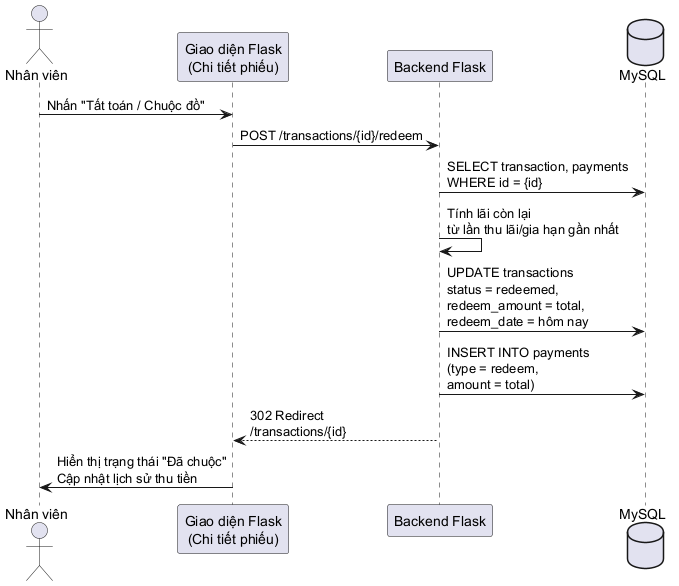
\includegraphics[width=\textwidth]{diagrams/pawnshop_sequence_redeem.png}
  \caption{Sơ đồ tuần tự nghiệp vụ tất toán / chuộc đồ}
  \label{fig:seq_redeem}
\end{figure}

\section{Sơ đồ tuần tự nghiệp vụ thu lãi bằng mã QR}

Bên cạnh nghiệp vụ tất toán, quy trình thu lãi kỳ bằng mã QR cũng là điểm nhấn của hệ thống vì giúp đơn giản hóa việc thu tiền và hạn chế sai sót trong khâu đếm tiền mặt. Hình~\ref{fig:seq_interest_qr} mô tả trình tự các thông điệp khi nhân viên sử dụng chức năng ``QR thanh toán lãi'' trên màn hình chi tiết phiếu. Đầu tiên, nhân viên bấm nút để hệ thống tính toán tiền lãi kỳ này, sinh đường dẫn ảnh QR từ dịch vụ VietQR và trả về một trang chuyên biệt hiển thị mã QR cùng số tiền cần thanh toán. Nhân viên đưa màn hình này cho khách hàng quét bằng ứng dụng ngân hàng trên điện thoại.

Sau khi khách hàng hoàn tất chuyển khoản, nhân viên quay lại giao diện và nhấn nút ``Xác nhận đã nhận tiền''. Giao diện lúc này gửi yêu cầu \texttt{POST /transactions/\{id\}/interest} đến backend. Backend kiểm tra lại thông tin phiếu, tính lãi lần nữa để bảo đảm dữ liệu nhất quán, sau đó ghi một bản ghi \texttt{Payment} loại ``interest'' vào cơ sở dữ liệu và chuyển hướng về trang chi tiết phiếu. Nhờ đó, lịch sử thu lãi được lưu trữ đầy đủ, đồng thời giao diện luôn phản ánh chính xác số tiền lãi đã thu và số ngày kể từ lần thu lãi gần nhất.

\begin{figure}[H]
  \centering
  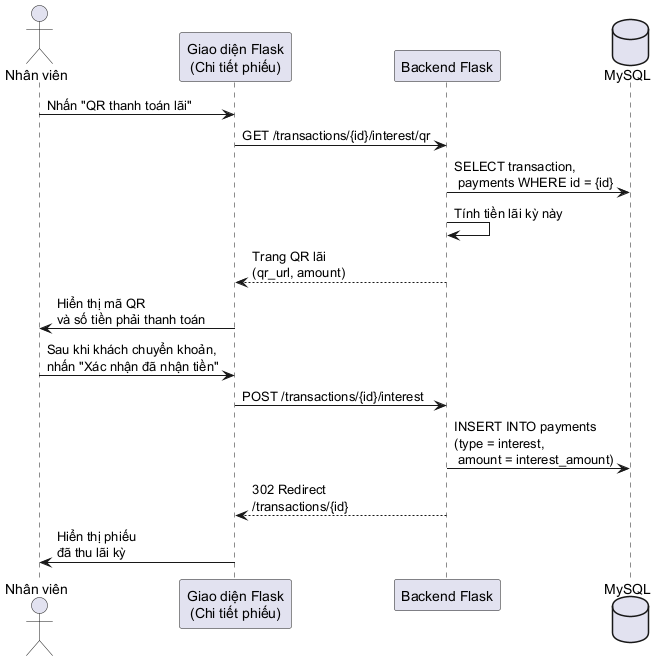
\includegraphics[width=\textwidth]{diagrams/pawnshop_sequence_interest_qr.png}
  \caption{Sơ đồ tuần tự nghiệp vụ thu lãi bằng mã QR}
  \label{fig:seq_interest_qr}
\end{figure}

\section{Sơ đồ tuần tự nghiệp vụ gia hạn phiếu}

Gia hạn phiếu là nghiệp vụ gắn liền với thu lãi định kỳ, cho phép khách hàng tiếp tục cầm tài sản sau khi đã thanh toán đầy đủ lãi kỳ trước. Hình~\ref{fig:seq_extend} trình bày trình tự các thông điệp khi nhân viên thực hiện gia hạn trên màn hình chi tiết phiếu. Đầu tiên, nhân viên nhấn nút ``Gia hạn'', giao diện gửi yêu cầu tới backend để tải lại thông tin phiếu và lịch sử thu tiền liên quan. Thông tin này giúp hệ thống xác định chính xác kỳ lãi cần thu và số lần gia hạn đã thực hiện.

Sau khi nhân viên nhập số ngày gia hạn và xác nhận, giao diện gửi yêu cầu \texttt{POST /transactions/\{id\}/extend} kèm theo tham số \texttt{extension\_days}. Backend kiểm tra trạng thái phiếu, tính lãi kỳ trước, ghi nhận một bản ghi \texttt{Payment} loại ``extension'' và cập nhật lại hạn chuộc cùng số lần gia hạn trong bảng \texttt{transactions}. Cuối cùng, hệ thống chuyển hướng về trang chi tiết phiếu với thông tin hạn chuộc mới và lịch sử thu tiền đã được bổ sung, giúp nhân viên và chủ tiệm dễ dàng theo dõi quá trình gia hạn của từng phiếu.

\begin{figure}[H]
  \centering
  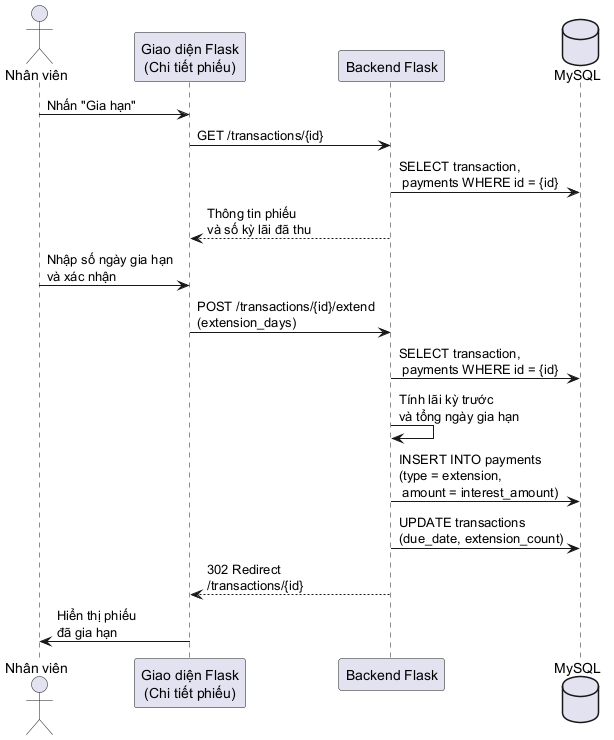
\includegraphics[width=\textwidth]{diagrams/pawnshop_sequence_extend.png}
  \caption{Sơ đồ tuần tự nghiệp vụ gia hạn phiếu cầm đồ}
  \label{fig:seq_extend}
\end{figure}

%---------------------------------------
\chapter{ĐÁNH GIÁ HỆ THỐNG}
%---------------------------------------

\section{Phương pháp đánh giá}

Việc đánh giá hệ thống được thực hiện theo hướng thực nghiệm, bám sát những nghiệp vụ quan trọng nhất của tiệm cầm đồ như lập phiếu cầm, thu lãi, gia hạn, tất toán, in phiếu, thanh toán bằng mã QR và lập báo cáo doanh thu. Em tiến hành cho người dùng thử là quản lý và nhân viên giao dịch thao tác trực tiếp trên hệ thống Flask, ghi nhận phản hồi, các lỗi phát sinh cũng như những đề xuất cải tiến giao diện. Quy trình kiểm thử được chia thành ba nhóm chính.

Nhóm thứ nhất là kiểm thử chức năng (functional testing). Các chức năng thêm, sửa, xóa khách hàng, lập phiếu cầm, thu lãi, gia hạn, tất toán, in phiếu, khóa/mở tài khoản nhân viên và xem báo cáo được thử với nhiều bộ dữ liệu khác nhau, bao gồm cả đầu vào hợp lệ, đầu vào biên và đầu vào không hợp lệ để quan sát cách hệ thống phản hồi. Đặc biệt, các quy tắc nghiệp vụ quan trọng như ``chỉ cho gia hạn khi phiếu chưa quá hạn'', ``chỉ cho thu lãi đúng ngày hạn'', ``phiếu đã chuộc không được tất toán lại'' được kiểm tra kỹ thông qua các kịch bản thử.

Nhóm thứ hai là kiểm thử tích hợp (integration testing), trong đó em kiểm tra sự đồng bộ giữa các module: khi lập phiếu mới, số liệu có xuất hiện ngay trên Dashboard và Báo cáo hay không; khi thu lãi hoặc gia hạn, lịch sử thu tiền có hiển thị đúng trong chi tiết phiếu và có ảnh hưởng chính xác đến phần lãi trong báo cáo doanh thu hay không; khi tất toán phiếu, trạng thái có chuyển sang ``Đã chuộc'' và không còn hiển thị trong danh sách phiếu đang cầm nữa. Các phép thử này giúp bảo đảm rằng dữ liệu được luân chuyển nhất quán giữa các bảng \texttt{transactions} và \texttt{payments}, cũng như giữa các màn hình giao diện khác nhau.

Nhóm thứ ba là kiểm thử trải nghiệm người dùng và hiệu năng ở quy mô nhỏ. Em nhập trước một lượng dữ liệu giả định gồm vài chục khách hàng, vài chục tài sản và hàng chục phiếu cầm để đánh giá tốc độ phản hồi của các màn hình tra cứu và lọc dữ liệu. Đồng thời, em quan sát cách người dùng thực tế thao tác với giao diện: liệu các nút chức năng có dễ nhận biết, các thông báo lỗi có rõ ràng, các con số tiền tệ có được định dạng nhất quán và dễ đọc hay không. Các góp ý về vị trí nút, màu sắc badge trạng thái, cách trình bày vùng nút xử lý trên màn hình chi tiết phiếu được ghi nhận và chỉnh sửa lại ngay trong quá trình phát triển.

\section{Kịch bản kiểm thử chức năng}

Bên cạnh việc mô tả phương pháp kiểm thử, đề tài còn xây dựng một số kịch bản kiểm thử hộp đen (blackbox) cho các chức năng quan trọng trên giao diện. Bảng~\ref{tab:test-functional} tổng hợp một số test case tiêu biểu cho các nghiệp vụ như đăng nhập, lập phiếu cầm, thu lãi, gia hạn, tất toán và xem báo cáo. Mỗi test case mô tả dữ liệu đầu vào, các bước thực hiện và kết quả mong đợi để có thể lặp lại quá trình kiểm thử khi cần.

\begin{table}[H]
\centering
\caption{Bảng kiểm thử chức năng nghiệp vụ chính}
\label{tab:test-functional}
\resizebox{\textwidth}{!}{%
\begin{tabular}{p{0.8cm}p{3.2cm}p{3.5cm}p{4.2cm}p{4.3cm}}
\hline
STT & Chức năng & Dữ liệu đầu vào & Bước thực hiện & Kết quả mong đợi \\
\hline
1 & Đăng nhập hệ thống & Tên đăng nhập hợp lệ, mật khẩu đúng & Mở trang đăng nhập, nhập thông tin và nhấn ``Đăng nhập'' & Hệ thống cho phép vào Dashboard, hiển thị tên người dùng ở góc trên bên phải \\
2 & Đăng nhập thất bại & Tên đăng nhập đúng, mật khẩu sai & Mở trang đăng nhập, nhập mật khẩu sai và nhấn ``Đăng nhập'' & Hệ thống giữ nguyên trang đăng nhập và hiển thị thông báo lỗi ``Sai tên đăng nhập hoặc mật khẩu'' \\
3 & Lập phiếu cầm hợp lệ & Khách hàng đã tồn tại, thông tin tài sản đầy đủ, số tiền và lãi suất hợp lệ & Từ màn hình Giao dịch, nhấn ``Lập phiếu cầm'', chọn khách hàng, nhập thông tin tài sản, số tiền, lãi suất, hạn chuộc và lưu & Phiếu cầm mới được tạo, hiện trong danh sách với trạng thái ``Đang cầm'' \\
4 & Thu lãi đúng hạn & Phiếu đang ở trạng thái ``Đang cầm'', ngày hiện tại trùng với ngày hạn đóng lãi & Mở chi tiết phiếu, nhấn ``Thu lãi'', xác nhận số tiền lãi kỳ này & Hệ thống ghi một bản ghi \texttt{Payment} loại ``interest'' và cập nhật số ngày kể từ lần thu lãi gần nhất về 0 \\
5 & Thu lãi sai thời điểm & Phiếu ở trạng thái ``Đang cầm'', ngày hiện tại trước ngày hạn đóng lãi & Mở chi tiết phiếu, nhấn ``Thu lãi'' & Hệ thống hiển thị thông báo lỗi về thời điểm thu lãi, không tạo bản ghi thanh toán mới \\
6 & Gia hạn hợp lệ & Phiếu ``Đang cầm'' hoặc ``Đã gia hạn'', chưa quá hạn & Mở chi tiết phiếu, nhấn ``Gia hạn'', nhập số ngày gia hạn và xác nhận & Hệ thống tính lãi kỳ trước, tạo bản ghi \texttt{Payment} loại ``extension'', cập nhật hạn chuộc mới và số lần gia hạn \\
7 & Tất toán phiếu & Phiếu đang ở trạng thái ``Đang cầm'' hoặc ``Đã gia hạn'' & Mở chi tiết phiếu, nhấn ``Tất toán / Chuộc đồ'', xác nhận số tiền gốc và lãi còn lại & Hệ thống ghi bản ghi \texttt{Payment} loại ``redeem'', cập nhật trạng thái phiếu sang ``Đã chuộc'' và không còn hiển thị trong danh sách phiếu đang cầm \\
8 & Xem báo cáo doanh thu & Dữ liệu \texttt{transactions} và \texttt{payments} trong một năm nhất định & Mở màn hình Báo cáo, chọn năm và nhấn ``Xem'' & Hệ thống hiển thị biểu đồ doanh thu theo tháng và bảng chi tiết tổng tiền gốc đã chuộc, tổng tiền lãi đã thu tương ứng \\
\hline
\end{tabular}
}%
\end{table}

Ngoài các test case hộp đen theo chức năng giao diện, đề tài còn xây dựng một số test case dạng hộp trắng đơn giản cho hàm tính lãi, nhằm kiểm tra tính đúng đắn của công thức tính lãi theo ngày trên một khoảng thời gian nhất định. Bảng~\ref{tab:test-interest} minh họa một vài trường hợp điển hình.

\begin{table}[H]
\centering
\caption{Bảng kiểm thử hàm tính lãi theo ngày}
\label{tab:test-interest}
\resizebox{\textwidth}{!}{%
\begin{tabular}{p{0.8cm}p{2.5cm}p{2.5cm}p{2.5cm}p{2.8cm}p{4.7cm}}
\hline
STT & Ngày bắt đầu & Ngày kết thúc & Lãi suất/tháng & Số tiền gốc & Kết quả mong đợi \\
\hline
1 & 01/01/2026 & 31/01/2026 & 3\% & 10.000.000 & Tiền lãi = 10.000.000 $\times$ 3\% = 300.000 đồng \\
2 & 01/01/2026 & 16/01/2026 & 3\% & 10.000.000 & Tiền lãi = 10.000.000 $\times$ 3\% $\times$ 15/30 = 150.000 đồng \\
3 & 10/02/2026 & 10/03/2026 & 4\% & 5.000.000 & Tiền lãi = 5.000.000 $\times$ 4\% = 200.000 đồng \\
4 & 01/03/2026 & 05/03/2026 & 3\% & 8.000.000 & Tiền lãi = 8.000.000 $\times$ 3\% $\times$ 4/30, làm tròn theo quy tắc của hệ thống \\
\hline
\end{tabular}
}%
\end{table}

\section{Kết quả đánh giá}

Qua quá trình thao tác thử nghiệm, hệ thống đáp ứng tương đối đầy đủ các yêu cầu đã đặt ra. Các lỗi phát hiện chủ yếu thuộc nhóm giao diện như văn bản hiển thị, căn lề, biểu tượng và một vài ngoại lệ chưa xử lý hết trong giai đoạn đầu; những vấn đề này đã được nhóm chỉnh sửa lại mã nguồn sau mỗi vòng kiểm thử. Các chức năng quản lý khách hàng, tài sản, lập phiếu cầm, thu lãi, gia hạn, tất toán và quản lý nhân viên hoạt động ổn định, dữ liệu được lưu trữ và truy vấn đúng. Màn hình chi tiết phiếu hiển thị rõ ràng trạng thái, lịch sử thu tiền, số ngày và số tiền lãi, giúp nhân viên dễ dàng giải thích cho khách hàng về khoản phải trả.

Module thanh toán qua mã QR VietQR hoạt động đúng như thiết kế: hệ thống sinh mã QR với số tiền và nội dung chuyển khoản phù hợp cho từng phiếu, hỗ trợ tốt cho các khách hàng có nhu cầu thanh toán chuyển khoản thay vì tiền mặt. Các mẫu phiếu cầm và phiếu chuộc được in trực tiếp từ hệ thống, bảo đảm tính thống nhất về bố cục và thông tin so với dữ liệu lưu trong cơ sở dữ liệu. Dashboard và màn hình báo cáo doanh thu hiển thị được tổng tiền gốc đã chuộc, tổng tiền lãi đã thu và biểu đồ doanh thu theo tháng, giúp quản lý dễ dàng theo dõi hiệu quả kinh doanh.

Tuy nhiên, quá trình đánh giá cũng cho thấy vẫn còn một số điểm cần cải thiện. Thứ nhất, hệ thống mới được thử nghiệm với dữ liệu ở quy mô thử nghiệm, chưa đánh giá hiệu năng khi số lượng phiếu cầm và lịch sử thu tiền tăng lên hàng chục nghìn bản ghi. Thứ hai, cơ chế phân quyền hiện tại dựa trên hai vai trò chính là quản lý và nhân viên, chưa hỗ trợ phân quyền chi tiết hơn theo từng chức năng nhỏ. Thứ ba, việc kiểm thử vẫn chủ yếu dựa trên thao tác thủ công; bộ kiểm thử tự động mới chỉ dừng ở script Selenium dùng để chụp hình minh họa, chưa bao phủ hết các kịch bản nghiệp vụ phức tạp.

%---------------------------------------
\chapter{KẾT LUẬN VÀ HƯỚNG PHÁT TRIỂN}
%---------------------------------------

\section{Kết luận}

Đề tài \emph{\TenDeTai} đã hiện thực một hệ thống quản lý tiệm cầm đồ chạy trên nền web với các module chính: quản lý khách hàng, quản lý tài sản cầm cố, lập phiếu cầm, thu lãi, gia hạn, tất toán, in phiếu, thanh toán qua mã QR, báo cáo doanh thu và quản lý nhân viên. Thông qua quá trình phân tích, thiết kế và triển khai, nhóm đã xây dựng được một giải pháp tương đối hoàn chỉnh cho bài toán quản lý tại một tiệm cầm đồ vừa và nhỏ, thay thế phần lớn các thao tác ghi chép sổ sách thủ công bằng quy trình điện tử rõ ràng, nhất quán và dễ kiểm soát.

So với mục tiêu đặt ra ban đầu, hệ thống đã đáp ứng được nhiều yêu cầu quan trọng. Về mặt nghiệp vụ, hệ thống bảo đảm tính toàn vẹn dữ liệu giữa phiếu cầm và lịch sử thu tiền, hỗ trợ quản lý khách hàng kèm giấy tờ tùy thân, thể hiện rõ vòng đời phiếu từ lúc lập, thu lãi, gia hạn cho đến tất toán, đồng thời cung cấp các báo cáo doanh thu gốc và lãi theo tháng. Các nghiệp vụ cốt lõi như lập phiếu, thu lãi, gia hạn, tất toán được chuẩn hóa thành những quy trình thao tác rõ ràng trên giao diện, giúp giảm phụ thuộc vào kinh nghiệm cá nhân của nhân viên và hạn chế nguy cơ sai sót trong tính toán thủ công.

Về mặt kỹ thuật, việc lựa chọn Flask kết hợp với SQLAlchemy và MySQL cho phép xây dựng một kiến trúc gọn nhẹ nhưng đủ linh hoạt để mở rộng về sau. Cách tổ chức mã nguồn theo mô hình gần với MVC, tách bạch giữa Model, View, Controller và các service tính toán, giúp hệ thống dễ bảo trì, dễ kiểm thử và dễ bổ sung chức năng mới. Sự kết hợp giữa TailwindCSS và các template Jinja2 giúp giao diện giữ được tính hiện đại, đồng thời dễ dàng chỉnh sửa khi có yêu cầu thay đổi từ phía người dùng.

Một điểm đáng ghi nhận khác là hệ thống đã đưa vào sử dụng một số đặc điểm phù hợp với xu hướng số hóa hiện nay như tích hợp thanh toán qua mã QR VietQR, in phiếu trực tiếp từ hệ thống với thông tin đồng nhất với dữ liệu lưu trong cơ sở dữ liệu, đồng thời hỗ trợ tự động chụp hình giao diện bằng Selenium để phục vụ công tác kiểm thử và lập tài liệu. Những yếu tố này cho thấy giải pháp không chỉ dừng lại ở mức đáp ứng tối thiểu bài toán quản lý mà còn hướng tới nâng cao trải nghiệm sử dụng và tính chuyên nghiệp trong hoạt động của tiệm cầm đồ.

\section{Hạn chế}

Mặc dù đã hoàn thành các chức năng cốt lõi, hệ thống vẫn còn một số hạn chế nhất định mà nhóm nhận thức rõ và xem như những hướng cải tiến cho giai đoạn tiếp theo. Trước hết, hệ thống hiện mới hỗ trợ mô hình một tiệm cầm đồ đơn lẻ, chưa quản lý được nhiều chi nhánh khác nhau. Toàn bộ nghiệp vụ được giả định diễn ra trong cùng một địa điểm, nên chưa giải quyết các bài toán phức tạp như phân bổ hạn mức vốn giữa các chi nhánh, tổng hợp báo cáo toàn hệ thống hay đồng bộ dữ liệu khi mất kết nối mạng. Điều này là hợp lý trong phạm vi đề tài, nhưng khi tiệm muốn mở rộng quy mô thì kiến trúc hiện tại sẽ cần được điều chỉnh để hỗ trợ tốt hơn mô hình phân tán.

Thứ hai, cơ chế phân quyền còn tương đối đơn giản, chủ yếu phân biệt giữa hai vai trò quản lý và nhân viên. Trong thực tế, một số tiệm cầm đồ có thể cần phân quyền chi tiết hơn, ví dụ phân biệt giữa nhân viên thu ngân, nhân viên tư vấn, nhân viên quản lý kho tài sản hoặc hạn chế một số thao tác nhạy cảm như sửa lãi suất, thay đổi hạn chuộc chỉ dành riêng cho một nhóm quản trị có thẩm quyền cao hơn. Việc mở rộng phân quyền theo hướng phân tách theo chức năng và theo phạm vi dữ liệu sẽ giúp hệ thống an toàn hơn và phù hợp với mô hình vận hành đa dạng ở các tiệm khác nhau.

Cuối cùng, hệ thống chưa được kiểm thử hiệu năng với dữ liệu rất lớn hoặc trong môi trường có nhiều người dùng truy cập đồng thời. Quy trình kiểm thử hiện chủ yếu dựa trên thao tác thủ công, chỉ dùng Selenium để mô phỏng một số kịch bản giao diện cơ bản, chưa có bộ kiểm thử tự động bao phủ hết các luồng nghiệp vụ phức tạp. Điều này khiến chi phí kiểm thử lại khi thay đổi chức năng còn phụ thuộc nhiều vào sức người, đồng thời chưa đánh giá được ngưỡng hiệu năng tối đa mà hệ thống có thể đáp ứng trong các tình huống tải cao.

\section{Hướng phát triển}

Trong tương lai, hệ thống có thể được mở rộng theo nhiều hướng khác nhau cả về nghiệp vụ lẫn kỹ thuật. Một hướng quan trọng là hỗ trợ đa chi nhánh, bổ sung các bảng và màn hình quản lý chi nhánh, cho phép cấu hình lãi suất và chính sách cầm khác nhau cho từng chi nhánh, đồng thời tổng hợp báo cáo doanh thu toàn hệ thống. Khi đó, kiến trúc triển khai có thể được nâng cấp theo hướng sử dụng một máy chủ ứng dụng trung tâm hoặc hạ tầng cloud, trong đó mỗi chi nhánh chỉ đóng vai trò là điểm truy cập qua trình duyệt, còn toàn bộ dữ liệu được lưu trữ tập trung trên một cụm cơ sở dữ liệu được sao lưu và giám sát chặt chẽ.

Một hướng phát triển khác là tích hợp sâu hơn với các dịch vụ bên thứ ba như cổng thanh toán ngân hàng, ví điện tử hoặc các nền tảng thanh toán QR nâng cao. Thay vì chỉ dừng lại ở việc sinh mã QR tĩnh, hệ thống có thể gửi yêu cầu tạo hóa đơn thanh toán trực tiếp tới ngân hàng và nhận callback khi giao dịch hoàn tất, từ đó tự động cập nhật trạng thái phiếu mà không cần nhân viên xác nhận thủ công. Điều này góp phần giảm rủi ro sai sót khi nhập liệu, đồng thời tạo trải nghiệm thanh toán hiện đại và tiện lợi hơn cho khách hàng.

Về phía khách hàng, module chăm sóc khách hàng có thể được mở rộng bằng cách xây dựng chức năng gửi SMS hoặc email tự động khi phiếu sắp đến hạn, khi khách có phiếu quá hạn hoặc khi tiệm triển khai chương trình ưu đãi. Trên nền tảng đó, hệ thống có thể kết hợp thêm một số thuật toán phân tích dữ liệu đơn giản để nhận diện nhóm khách hàng thường xuyên, khách hàng có nguy cơ không chuộc đồ hoặc khách hàng mang lại lợi nhuận cao, qua đó hỗ trợ chủ tiệm trong việc đưa ra các quyết định về chính sách lãi suất, thời hạn cầm và chương trình chăm sóc khách hàng phù hợp.

Về mặt kỹ thuật, hệ thống nên được bổ sung bộ kiểm thử tự động cho các controller Flask và các service quan trọng, kết hợp với pipeline CI/CD khi triển khai trên môi trường server thực tế. Việc áp dụng kiểm thử tự động và CI/CD giúp phát hiện sớm lỗi phát sinh khi mở rộng chức năng, giảm thiểu rủi ro khi cập nhật hệ thống trong môi trường đang vận hành. Trên nền tảng đó, nhóm có thể tiếp tục phát triển thêm các client khác như ứng dụng di động dành cho chủ tiệm hoặc cho nhân viên đi thu lãi bên ngoài, cho phép theo dõi tình hình phiếu cầm và doanh thu ở bất kỳ đâu chỉ với một thiết bị kết nối internet.

%---------------------------------------
\clearpage
\chapter*{TÀI LIỆU THAM KHẢO}
\addcontentsline{toc}{chapter}{TÀI LIỆU THAM KHẢO}
%---------------------------------------

[1] Miguel Grinberg, \emph{Flask Web Development}. O'Reilly Media, 2018.
 
[2] Pallets Projects, \emph{Flask Documentation}.  
Truy cập tại: \href{https://flask.palletsprojects.com}{https://flask.palletsprojects.com}.
 
[3] SQLAlchemy, \emph{SQLAlchemy 2.0 Documentation}.  
Truy cập tại: \href{https://docs.sqlalchemy.org}{https://docs.sqlalchemy.org}.
 
[4] Selenium Project, \emph{Selenium WebDriver Documentation}.  
Truy cập tại: \href{https://www.selenium.dev/documentation}{https://www.selenium.dev/documentation}.
 
[4] Oracle, \emph{MySQL 8.0 Reference Manual}.  
Truy cập tại: \href{https://dev.mysql.com/doc}{https://dev.mysql.com/doc}.
 
[5] Tailwind Labs, \emph{Tailwind CSS Documentation}.  
Truy cập tại: \href{https://tailwindcss.com/docs}{https://tailwindcss.com/docs}.
 
[6] Chart.js, \emph{Chart.js Documentation}.  
Truy cập tại: \href{https://www.chartjs.org/docs}{https://www.chartjs.org/docs}.
 

\end{document}
